\chapter{The reference file}
\section{The source text}
This is the file we will use to check the prototype. 
It will be FTP'd from one machine to another.
\begin{chunk}{reference.java}
import java.io.IOException;
import java.util.ArrayList;
import java.util.Collection;
import java.util.List;
import org.apache.commons.configuration.ConfigurationException;
import org.apache.uima.UimaContext;
import org.apache.uima.analysis_component.JCasAnnotator_ImplBase;
import org.apache.uima.analysis_engine.AnalysisEngineProcessException;
import org.apache.uima.cas.FSIterator;
import org.apache.uima.jcas.JCas;
import org.apache.uima.jcas.cas.FSList;
import org.apache.uima.jcas.cas.StringList;
import org.apache.uima.resource.ResourceInitializationException;
import util.*;
import edu.cmu.lti.oaqa.bio.bioasq.services.GoPubMedService;
import edu.cmu.lti.oaqa.bio.bioasq.services.LinkedLifeDataServiceResponse;
import edu.cmu.lti.oaqa.bio.bioasq.services.OntologyServiceResponse;
import edu.cmu.lti.oaqa.bio.bioasq.services.PubMedSearchServiceResponse;
import edu.cmu.lti.oaqa.bio.bioasq.services.PubMedSearchServiceResponse.Document;
import edu.cmu.lti.oaqa.type.input.Question;
import edu.cmu.lti.oaqa.type.kb.Concept;
import edu.cmu.lti.oaqa.type.kb.Triple;

public class Annotator extends JCasAnnotator_ImplBase {
  static GoPubMedService service = null;

  @Override
  public void initialize(UimaContext aContext) throws ResourceInitializationException {
    try {
      GoPubMedService service = new GoPubMedService("./project.properties");
    } catch (ConfigurationException e) {
      // TODO Auto-generated catch block
      e.printStackTrace();
    }
  }

  @Override
  public void process(JCas aJCas) throws AnalysisEngineProcessException {
    // TODO Auto-generated method stub
    FSIterator it = aJCas.getAnnotationIndex(Question.type).iterator();
    // String Doc = aJCas.getDocumentText();
    Question questionTypeSys = null;
    if (it.hasNext()) {
      questionTypeSys = (Question) it.next();
    }
    String text = questionTypeSys.getText();
    Concept conceptTypeSys = null;
    // StringList conceptStringList = null;
    // FSList mentionList = null;
    List<String> conceptList = null;
    List<Double> confidenceList = null;
    edu.cmu.lti.oaqa.type.retrieval.Document documentTypeSys = null;
    // StringList documentStringList = null;
    Triple tripleTypeSys = null;
    try {
      OntologyServiceResponse.Result diseaseOntologyResult = service
              .findDiseaseOntologyEntitiesPaged(text, 0);
      conceptList = new ArrayList<String>();
      confidenceList = new ArrayList<Double>();
      conceptTypeSys = new Concept(aJCas);
      for (OntologyServiceResponse.Finding finding : diseaseOntologyResult.getFindings()) {
        conceptList.add(finding.getConcept().getUri());
        confidenceList.add(finding.getScore());
      }
      conceptTypeSys.setName("Disease Ontology");
      //conceptTypeSys.setUris(Utils.createStringList(aJCas, conceptList));
      //conceptTypeSys.setMentions(Utils.fromCollectionToFSList(aJCas, (Collection) confidenceList));
      conceptTypeSys.addToIndexes(aJCas);
      conceptList = new ArrayList<String>();
      confidenceList = new ArrayList<Double>();
      conceptTypeSys = new Concept(aJCas);
      OntologyServiceResponse.Result geneOntologyResult = service.findGeneOntologyEntitiesPaged(
              text, 0, 10);
      for (OntologyServiceResponse.Finding finding : geneOntologyResult.getFindings()) {
        conceptList.add(finding.getConcept().getUri());
        confidenceList.add(finding.getScore());
      }
      conceptTypeSys.setName("Gene Ontology");
      //conceptTypeSys.setUris(Utils.createStringList(aJCas, conceptList));
      //conceptTypeSys.setMentions(Utils.fromCollectionToFSList(aJCas, (Collection) confidenceList));
      conceptTypeSys.addToIndexes(aJCas);
      conceptList = new ArrayList<String>();
      confidenceList = new ArrayList<Double>();
      conceptTypeSys = new Concept(aJCas);
      OntologyServiceResponse.Result jochemResult = service.findJochemEntitiesPaged(text, 0);
      for (OntologyServiceResponse.Finding finding : jochemResult.getFindings()) {
        conceptList.add(finding.getConcept().getUri());
        confidenceList.add(finding.getScore());
      }
      conceptTypeSys.setName("Jochem");
      //conceptTypeSys.setUris(Utils.createStringList(aJCas, conceptList));
      //conceptTypeSys.setMentions(Utils.fromCollectionToFSList(aJCas, (Collection) confidenceList));
      conceptTypeSys.addToIndexes(aJCas);
      conceptList = new ArrayList<String>();
      confidenceList = new ArrayList<Double>();
      conceptTypeSys = new Concept(aJCas);
      OntologyServiceResponse.Result meshResult = service.findMeshEntitiesPaged(text, 0);
      for (OntologyServiceResponse.Finding finding : meshResult.getFindings()) {
        conceptList.add(finding.getConcept().getUri());
        confidenceList.add(finding.getScore());
      }
      conceptTypeSys.setName("MeSH");
      //conceptTypeSys.setUris(Utils.createStringList(aJCas, conceptList));
      //conceptTypeSys.setMentions(Utils.fromCollectionToFSList(aJCas, (Collection) confidenceList));
      conceptTypeSys.addToIndexes(aJCas);
      conceptList = new ArrayList<String>();
      confidenceList = new ArrayList<Double>();
      conceptTypeSys = new Concept(aJCas);
      OntologyServiceResponse.Result uniprotResult = service.findUniprotEntitiesPaged(text, 0);
      for (OntologyServiceResponse.Finding finding : uniprotResult.getFindings()) {
        conceptList.add(finding.getConcept().getUri());
        confidenceList.add(finding.getScore());
      }
      conceptTypeSys.setName("UniProt");
      //conceptTypeSys.setUris(Utils.createStringList(aJCas, conceptList));
      //conceptTypeSys.setMentions(Utils.fromCollectionToFSList(aJCas, (Collection) confidenceList));
      conceptTypeSys.addToIndexes(aJCas);
      // Triples
      LinkedLifeDataServiceResponse.Result linkedLifeDataResult = service
              .findLinkedLifeDataEntitiesPaged(text, 0);
      // System.out.println("LinkedLifeData: " + linkedLifeDataResult.getEntities().size());
      for (LinkedLifeDataServiceResponse.Entity entity : linkedLifeDataResult.getEntities()) {
        // System.out.println(" > " + entity.getEntity());
        for (LinkedLifeDataServiceResponse.Relation relation : entity.getRelations()) {
          tripleTypeSys = new Triple(aJCas);
          tripleTypeSys.setObject(relation.getObj());
          tripleTypeSys.setSubject(relation.getSubj());
          tripleTypeSys.setPredicate(relation.getPred());
          tripleTypeSys.addToIndexes(aJCas);
        }
      }
      PubMedSearchServiceResponse.Result pubmedResult = service.findPubMedCitations(text, 0);
      List<Document> docList = pubmedResult.getDocuments();
      // String[] pmids = new String[docList.size()];
      // int i = 0;
      for (Document doc : docList) {
        documentTypeSys = new edu.cmu.lti.oaqa.type.retrieval.Document(aJCas);
        documentTypeSys.setTitle("http://www.ncbi.nlm.nih.gov/pubmed/" + doc.getPmid());
        documentTypeSys.setDocId(doc.getPmid());
        documentTypeSys.addToIndexes(aJCas);
        // documentTypeSys.setDocId(doc);
        // pmids[i++] = "http://www.ncbi.nlm.nih.gov/pubmed/" + doc.getPmid();
        // System.out.println( pmids[i - 1]);
      }
    } catch (IOException e) {
      // TODO Auto-generated catch block
      e.printStackTrace();
    }
  }
}
\end{chunk}

\newpage
\section{The FTP packet frames}
These are the bytes transmitted on the wire (captured by wireshark)
during the FTP transfer. 

\begin{figure}[ht!]
\centering
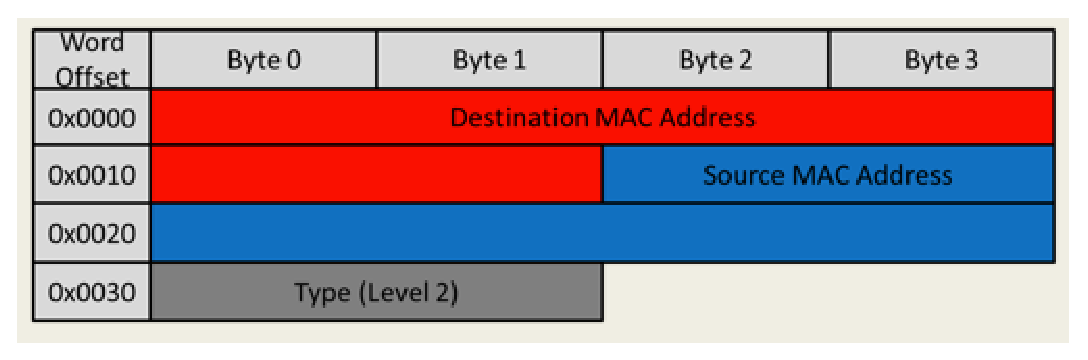
\includegraphics[scale=0.75]{eps/level1Header.eps}
\caption{The Level 1 Ethernet Header\cite{37}}
\label{level1Header}
\end{figure}
 
\vspace{1mm}
\noindent
{\bf The Destination MAC address}
\begin{verbatim}
0000 -- 0xd4, 0xbe, 0xd9, 0x50, 0xfa, 0xb2,             /* ...P..@< */
\end{verbatim}
That is, D4:BE:D9:50:FA:B2

\vspace{1mm}
\noindent
{\bf The Source MAC address}
\begin{verbatim}
0000 --                                     0x40, 0x3c, /* ...P..@< */
0008 -- 0xfc, 0x01, 0x04, 0x85,                         /* ......E. */
\end{verbatim}
That is, 40:3C:FC:01:04:85

\vspace{1mm}
\noindent
{\bf Type} 
\begin{verbatim}
0008 --                         0x08, 0x00,             /* ......E. */
\end{verbatim}
If the type field of the Ethernet header contains 0x0800 (which
this does) there will be a second nested level. The contents of
this level are described by the IP header. 

\begin{figure}[ht!]
\centering
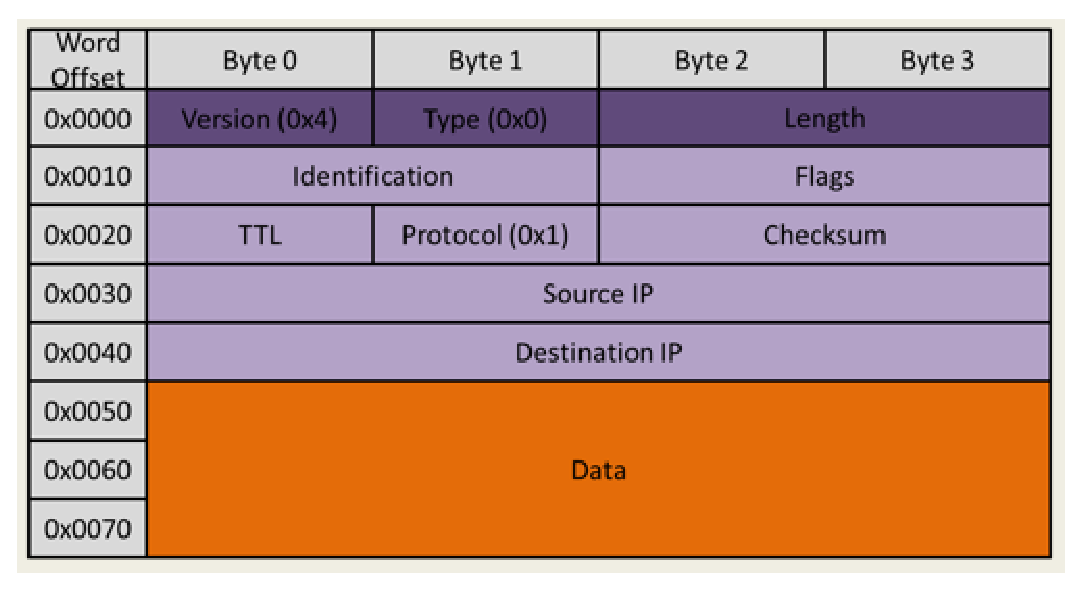
\includegraphics[scale=0.75]{eps/level2Header.eps}
\caption{The Level 2 IP Ethernet Header\cite{37}}
\label{level2Header}
\end{figure}

\vspace{1mm}
\noindent
{\bf Version} (4 bits)
\begin{verbatim}
0008 --                                     0x4 ,       /* ......E. */
\end{verbatim}
The Version is 4, which signals IPv4

\vspace{1mm}
\noindent
{\bf Internet Header Length} (4 bits)
\begin{verbatim}
0008 --                                       0x 5,     /* ......E. */
\end{verbatim}
The Internet Header Length is 5, which means 5x32 = 160 bits =20 bytes

\vspace{1mm}
\noindent
{\bf Type of Service} (1 byte)
\begin{verbatim}
0008 --                                           0x08, /* ......E. */
\end{verbatim}
This field is actually 2 fields, a 6-bit Differentiated Servies Code Point
and and Explicit Congestion Notification (2 bit). \cite{41}

\vspace{1mm}
\noindent
{\bf Total Length} (2 bytes)
\begin{verbatim}
0010 -- 0x05, 0xdc,                                     /* ..rD@.@. */
\end{verbatim}
Hex 0x5DC = 1500

\vspace{1mm}
\noindent
{\bf Identification} (2 bytes)
\begin{verbatim}
0010 --             0x72, 0x44,                         /* ..rD@.@. */
\end{verbatim}
The identiication field is primarily used for uniquely identifying the
group of fragments of a single IP datagram. \cite{41}

\vspace{1mm}
\noindent
{\bf Flags} (3 bits)
\begin{verbatim}
0010 --                         0x4                     /* ..rD@.@. */
0010 --                         0x 0, 0x00              /* ..rD@.@. */
\end{verbatim}
This 3-bit field is used to control or identify fragments.
This has the Don't Fragment (DF) bit set.\cite{41}

\vspace{1mm}
\noindent
{\bf Fragmentation Offset} (13 bits)
\begin{verbatim}
0010 --                         0x 0, 0x00              /* ..rD@.@. */
\end{verbatim}
The packet is not fragmented so there is no offset.

\vspace{1mm}
\noindent
{\bf Time to Live} (1 byte)
\begin{verbatim}
0010 --                                     0x40        /* ..rD@.@. */
\end{verbatim}
Supposed to be a number of seconds but is usually a hop count.

\vspace{1mm}
\noindent
{\bf Protocol} (1 bytes) \cite{43}
\begin{verbatim}
0010 --                                           0x06, /* ..rD@.@. */
\end{verbatim}
The 6 identifies this as a TCP packet. Note the FTP is a TCP-based
protocol.

\vspace{1mm}
\noindent
{\bf Header Checksum} (2 bytes)
\begin{verbatim}
0018 -- 0x3f, 0x7c, 0xc0, 0xa8                          /* ?|...... */
\end{verbatim}
0x3F7CC0A8 = 1065140392

\vspace{1mm}
\noindent
RFC 1071 defines the checksum calculation:

The checksum field is the 16-bit one's complement of the one's
complement sum of all 16-bit words in the header. For purposes of
computing the checksum, the value of the checksum field is zero.

\vspace{1mm}
\noindent
For example, consider 
\begin{verbatim} 
Hex 4500003044224000800600008c7c19acae241e2b
\end{verbatim}
(20 bytes IP header), using a machine which uses standard two's 
complement arithmetic:
\begin{enumerate}
\item 4500 + 0030 + 4422 + 4000 + 8006 + 0000 + 8c7c + 19ac + ae24 + 1e2b =
 0002BBCF (32-bit sum)
\item 0002 + BBCF = BBD1 = 1011101111010001 (1's complement 16-bit sum, 
formed by ``end around carry'' of 32-bit 2's complement sum)
\item ~BBD1 = 0100010000101110 = 442E (1's complement of 1's complement 
16-bit sum)
\end{enumerate}
To validate a header's checksum the same algorithm may be used - the 
checksum of a header which contains a correct checksum field is a word 
containing all zeros (value 0):
\begin{verbatim}
2BBCF + 442E = 2FFFD. 2 + FFFD = FFFF. the 1's complement of FFFF = 0.
\end{verbatim}

\vspace{1mm}
\noindent
{\bf The Source Address} (4 bytes)
\begin{verbatim}
0018 --                         0x01, 0x02, 0xc0, 0xa8, /* ?|...... */
\end{verbatim}
This is 192.168.1.2

\vspace{1mm}
\noindent
{\bf The Destination Address} (4 bytes)
\begin{verbatim}
0020 -- 0x01, 0x01, 0x00, 0x14,                         /* .....u.. */
\end{verbatim}
This appears to be 0.20.1.1 (which is nonsense)

\vspace{1mm}
\noindent
These bytes still need to be explained:
\begin{verbatim}
0020 --                         0xdf, 0x75, 0xe1, 0x89, /* .....u.. */
0028 -- 0xc7, 0x42, 0x28, 0x0a, 0x7e, 0xea, 0x80, 0x10, /* .B(.~... */
0030 -- 0x01, 0xc9, 0x8b, 0x61, 0x00, 0x00, 0x01, 0x01, /* ...a.... */
\end{verbatim}

\vspace{1mm}
\noindent
The {\bf Data} packet (offset x42)
\begin{verbatim}
  i     m     p     o     r     t
0042 -- 0x69, 0x6d, 0x70, 0x6f, 0x72, 0x74, /* import */
\end{verbatim}
The data packet length is 1514-66=1448 bytes (x42=66, the header length).

\begin{chunk}{referenceFrames}
/* Frame (1514 bytes) */
static const unsigned char pkt11[1514] = {
0xd4, 0xbe, 0xd9, 0x50, 0xfa, 0xb2, 0x40, 0x3c, /* ...P..@< */
0xfc, 0x01, 0x04, 0x85, 0x08, 0x00, 0x45, 0x08, /* ......E. */
0x05, 0xdc, 0x72, 0x44, 0x40, 0x00, 0x40, 0x06, /* ..rD@.@. */
0x3f, 0x7c, 0xc0, 0xa8, 0x01, 0x02, 0xc0, 0xa8, /* ?|...... */
0x01, 0x01, 0x00, 0x14, 0xdf, 0x75, 0xe1, 0x89, /* .....u.. */
0xc7, 0x42, 0x28, 0x0a, 0x7e, 0xea, 0x80, 0x10, /* .B(.~... */
0x01, 0xc9, 0x8b, 0x61, 0x00, 0x00, 0x01, 0x01, /* ...a.... */
0x08, 0x0a, 0x00, 0xf8, 0xb5, 0x03, 0x00, 0x07, /* ........ */
0x27, 0x99, 0x69, 0x6d, 0x70, 0x6f, 0x72, 0x74, /* '.import */
0x20, 0x6a, 0x61, 0x76, 0x61, 0x2e, 0x69, 0x6f, /*  java.io */
0x2e, 0x49, 0x4f, 0x45, 0x78, 0x63, 0x65, 0x70, /* .IOExcep */
0x74, 0x69, 0x6f, 0x6e, 0x3b, 0x0a, 0x69, 0x6d, /* tion;.im */
0x70, 0x6f, 0x72, 0x74, 0x20, 0x6a, 0x61, 0x76, /* port jav */
0x61, 0x2e, 0x75, 0x74, 0x69, 0x6c, 0x2e, 0x41, /* a.util.A */
0x72, 0x72, 0x61, 0x79, 0x4c, 0x69, 0x73, 0x74, /* rrayList */
0x3b, 0x0a, 0x69, 0x6d, 0x70, 0x6f, 0x72, 0x74, /* ;.import */
0x20, 0x6a, 0x61, 0x76, 0x61, 0x2e, 0x75, 0x74, /*  java.ut */
0x69, 0x6c, 0x2e, 0x43, 0x6f, 0x6c, 0x6c, 0x65, /* il.Colle */
0x63, 0x74, 0x69, 0x6f, 0x6e, 0x3b, 0x0a, 0x69, /* ction;.i */
0x6d, 0x70, 0x6f, 0x72, 0x74, 0x20, 0x6a, 0x61, /* mport ja */
0x76, 0x61, 0x2e, 0x75, 0x74, 0x69, 0x6c, 0x2e, /* va.util. */
0x4c, 0x69, 0x73, 0x74, 0x3b, 0x0a, 0x69, 0x6d, /* List;.im */
0x70, 0x6f, 0x72, 0x74, 0x20, 0x6f, 0x72, 0x67, /* port org */
0x2e, 0x61, 0x70, 0x61, 0x63, 0x68, 0x65, 0x2e, /* .apache. */
0x63, 0x6f, 0x6d, 0x6d, 0x6f, 0x6e, 0x73, 0x2e, /* commons. */
0x63, 0x6f, 0x6e, 0x66, 0x69, 0x67, 0x75, 0x72, /* configur */
0x61, 0x74, 0x69, 0x6f, 0x6e, 0x2e, 0x43, 0x6f, /* ation.Co */
0x6e, 0x66, 0x69, 0x67, 0x75, 0x72, 0x61, 0x74, /* nfigurat */
0x69, 0x6f, 0x6e, 0x45, 0x78, 0x63, 0x65, 0x70, /* ionExcep */
0x74, 0x69, 0x6f, 0x6e, 0x3b, 0x0a, 0x69, 0x6d, /* tion;.im */
0x70, 0x6f, 0x72, 0x74, 0x20, 0x6f, 0x72, 0x67, /* port org */
0x2e, 0x61, 0x70, 0x61, 0x63, 0x68, 0x65, 0x2e, /* .apache. */
0x75, 0x69, 0x6d, 0x61, 0x2e, 0x55, 0x69, 0x6d, /* uima.Uim */
0x61, 0x43, 0x6f, 0x6e, 0x74, 0x65, 0x78, 0x74, /* aContext */
0x3b, 0x0a, 0x69, 0x6d, 0x70, 0x6f, 0x72, 0x74, /* ;.import */
0x20, 0x6f, 0x72, 0x67, 0x2e, 0x61, 0x70, 0x61, /*  org.apa */
0x63, 0x68, 0x65, 0x2e, 0x75, 0x69, 0x6d, 0x61, /* che.uima */
0x2e, 0x61, 0x6e, 0x61, 0x6c, 0x79, 0x73, 0x69, /* .analysi */
0x73, 0x5f, 0x63, 0x6f, 0x6d, 0x70, 0x6f, 0x6e, /* s_compon */
0x65, 0x6e, 0x74, 0x2e, 0x4a, 0x43, 0x61, 0x73, /* ent.JCas */
0x41, 0x6e, 0x6e, 0x6f, 0x74, 0x61, 0x74, 0x6f, /* Annotato */
0x72, 0x5f, 0x49, 0x6d, 0x70, 0x6c, 0x42, 0x61, /* r_ImplBa */
0x73, 0x65, 0x3b, 0x0a, 0x69, 0x6d, 0x70, 0x6f, /* se;.impo */
0x72, 0x74, 0x20, 0x6f, 0x72, 0x67, 0x2e, 0x61, /* rt org.a */
0x70, 0x61, 0x63, 0x68, 0x65, 0x2e, 0x75, 0x69, /* pache.ui */
0x6d, 0x61, 0x2e, 0x61, 0x6e, 0x61, 0x6c, 0x79, /* ma.analy */
0x73, 0x69, 0x73, 0x5f, 0x65, 0x6e, 0x67, 0x69, /* sis_engi */
0x6e, 0x65, 0x2e, 0x41, 0x6e, 0x61, 0x6c, 0x79, /* ne.Analy */
0x73, 0x69, 0x73, 0x45, 0x6e, 0x67, 0x69, 0x6e, /* sisEngin */
0x65, 0x50, 0x72, 0x6f, 0x63, 0x65, 0x73, 0x73, /* eProcess */
0x45, 0x78, 0x63, 0x65, 0x70, 0x74, 0x69, 0x6f, /* Exceptio */
0x6e, 0x3b, 0x0a, 0x69, 0x6d, 0x70, 0x6f, 0x72, /* n;.impor */
0x74, 0x20, 0x6f, 0x72, 0x67, 0x2e, 0x61, 0x70, /* t org.ap */
0x61, 0x63, 0x68, 0x65, 0x2e, 0x75, 0x69, 0x6d, /* ache.uim */
0x61, 0x2e, 0x63, 0x61, 0x73, 0x2e, 0x46, 0x53, /* a.cas.FS */
0x49, 0x74, 0x65, 0x72, 0x61, 0x74, 0x6f, 0x72, /* Iterator */
0x3b, 0x0a, 0x69, 0x6d, 0x70, 0x6f, 0x72, 0x74, /* ;.import */
0x20, 0x6f, 0x72, 0x67, 0x2e, 0x61, 0x70, 0x61, /*  org.apa */
0x63, 0x68, 0x65, 0x2e, 0x75, 0x69, 0x6d, 0x61, /* che.uima */
0x2e, 0x6a, 0x63, 0x61, 0x73, 0x2e, 0x4a, 0x43, /* .jcas.JC */
0x61, 0x73, 0x3b, 0x0a, 0x69, 0x6d, 0x70, 0x6f, /* as;.impo */
0x72, 0x74, 0x20, 0x6f, 0x72, 0x67, 0x2e, 0x61, /* rt org.a */
0x70, 0x61, 0x63, 0x68, 0x65, 0x2e, 0x75, 0x69, /* pache.ui */
0x6d, 0x61, 0x2e, 0x6a, 0x63, 0x61, 0x73, 0x2e, /* ma.jcas. */
0x63, 0x61, 0x73, 0x2e, 0x46, 0x53, 0x4c, 0x69, /* cas.FSLi */
0x73, 0x74, 0x3b, 0x0a, 0x69, 0x6d, 0x70, 0x6f, /* st;.impo */
0x72, 0x74, 0x20, 0x6f, 0x72, 0x67, 0x2e, 0x61, /* rt org.a */
0x70, 0x61, 0x63, 0x68, 0x65, 0x2e, 0x75, 0x69, /* pache.ui */
0x6d, 0x61, 0x2e, 0x6a, 0x63, 0x61, 0x73, 0x2e, /* ma.jcas. */
0x63, 0x61, 0x73, 0x2e, 0x53, 0x74, 0x72, 0x69, /* cas.Stri */
0x6e, 0x67, 0x4c, 0x69, 0x73, 0x74, 0x3b, 0x0a, /* ngList;. */
0x69, 0x6d, 0x70, 0x6f, 0x72, 0x74, 0x20, 0x6f, /* import o */
0x72, 0x67, 0x2e, 0x61, 0x70, 0x61, 0x63, 0x68, /* rg.apach */
0x65, 0x2e, 0x75, 0x69, 0x6d, 0x61, 0x2e, 0x72, /* e.uima.r */
0x65, 0x73, 0x6f, 0x75, 0x72, 0x63, 0x65, 0x2e, /* esource. */
0x52, 0x65, 0x73, 0x6f, 0x75, 0x72, 0x63, 0x65, /* Resource */
0x49, 0x6e, 0x69, 0x74, 0x69, 0x61, 0x6c, 0x69, /* Initiali */
0x7a, 0x61, 0x74, 0x69, 0x6f, 0x6e, 0x45, 0x78, /* zationEx */
0x63, 0x65, 0x70, 0x74, 0x69, 0x6f, 0x6e, 0x3b, /* ception; */
0x0a, 0x69, 0x6d, 0x70, 0x6f, 0x72, 0x74, 0x20, /* .import  */
0x75, 0x74, 0x69, 0x6c, 0x2e, 0x2a, 0x3b, 0x0a, /* util.*;. */
0x69, 0x6d, 0x70, 0x6f, 0x72, 0x74, 0x20, 0x65, /* import e */
0x64, 0x75, 0x2e, 0x63, 0x6d, 0x75, 0x2e, 0x6c, /* du.cmu.l */
0x74, 0x69, 0x2e, 0x6f, 0x61, 0x71, 0x61, 0x2e, /* ti.oaqa. */
0x62, 0x69, 0x6f, 0x2e, 0x62, 0x69, 0x6f, 0x61, /* bio.bioa */
0x73, 0x71, 0x2e, 0x73, 0x65, 0x72, 0x76, 0x69, /* sq.servi */
0x63, 0x65, 0x73, 0x2e, 0x47, 0x6f, 0x50, 0x75, /* ces.GoPu */
0x62, 0x4d, 0x65, 0x64, 0x53, 0x65, 0x72, 0x76, /* bMedServ */
0x69, 0x63, 0x65, 0x3b, 0x0a, 0x69, 0x6d, 0x70, /* ice;.imp */
0x6f, 0x72, 0x74, 0x20, 0x65, 0x64, 0x75, 0x2e, /* ort edu. */
0x63, 0x6d, 0x75, 0x2e, 0x6c, 0x74, 0x69, 0x2e, /* cmu.lti. */
0x6f, 0x61, 0x71, 0x61, 0x2e, 0x62, 0x69, 0x6f, /* oaqa.bio */
0x2e, 0x62, 0x69, 0x6f, 0x61, 0x73, 0x71, 0x2e, /* .bioasq. */
0x73, 0x65, 0x72, 0x76, 0x69, 0x63, 0x65, 0x73, /* services */
0x2e, 0x4c, 0x69, 0x6e, 0x6b, 0x65, 0x64, 0x4c, /* .LinkedL */
0x69, 0x66, 0x65, 0x44, 0x61, 0x74, 0x61, 0x53, /* ifeDataS */
0x65, 0x72, 0x76, 0x69, 0x63, 0x65, 0x52, 0x65, /* erviceRe */
0x73, 0x70, 0x6f, 0x6e, 0x73, 0x65, 0x3b, 0x0a, /* sponse;. */
0x69, 0x6d, 0x70, 0x6f, 0x72, 0x74, 0x20, 0x65, /* import e */
0x64, 0x75, 0x2e, 0x63, 0x6d, 0x75, 0x2e, 0x6c, /* du.cmu.l */
0x74, 0x69, 0x2e, 0x6f, 0x61, 0x71, 0x61, 0x2e, /* ti.oaqa. */
0x62, 0x69, 0x6f, 0x2e, 0x62, 0x69, 0x6f, 0x61, /* bio.bioa */
0x73, 0x71, 0x2e, 0x73, 0x65, 0x72, 0x76, 0x69, /* sq.servi */
0x63, 0x65, 0x73, 0x2e, 0x4f, 0x6e, 0x74, 0x6f, /* ces.Onto */
0x6c, 0x6f, 0x67, 0x79, 0x53, 0x65, 0x72, 0x76, /* logyServ */
0x69, 0x63, 0x65, 0x52, 0x65, 0x73, 0x70, 0x6f, /* iceRespo */
0x6e, 0x73, 0x65, 0x3b, 0x0a, 0x69, 0x6d, 0x70, /* nse;.imp */
0x6f, 0x72, 0x74, 0x20, 0x65, 0x64, 0x75, 0x2e, /* ort edu. */
0x63, 0x6d, 0x75, 0x2e, 0x6c, 0x74, 0x69, 0x2e, /* cmu.lti. */
0x6f, 0x61, 0x71, 0x61, 0x2e, 0x62, 0x69, 0x6f, /* oaqa.bio */
0x2e, 0x62, 0x69, 0x6f, 0x61, 0x73, 0x71, 0x2e, /* .bioasq. */
0x73, 0x65, 0x72, 0x76, 0x69, 0x63, 0x65, 0x73, /* services */
0x2e, 0x50, 0x75, 0x62, 0x4d, 0x65, 0x64, 0x53, /* .PubMedS */
0x65, 0x61, 0x72, 0x63, 0x68, 0x53, 0x65, 0x72, /* earchSer */
0x76, 0x69, 0x63, 0x65, 0x52, 0x65, 0x73, 0x70, /* viceResp */
0x6f, 0x6e, 0x73, 0x65, 0x3b, 0x0a, 0x69, 0x6d, /* onse;.im */
0x70, 0x6f, 0x72, 0x74, 0x20, 0x65, 0x64, 0x75, /* port edu */
0x2e, 0x63, 0x6d, 0x75, 0x2e, 0x6c, 0x74, 0x69, /* .cmu.lti */
0x2e, 0x6f, 0x61, 0x71, 0x61, 0x2e, 0x62, 0x69, /* .oaqa.bi */
0x6f, 0x2e, 0x62, 0x69, 0x6f, 0x61, 0x73, 0x71, /* o.bioasq */
0x2e, 0x73, 0x65, 0x72, 0x76, 0x69, 0x63, 0x65, /* .service */
0x73, 0x2e, 0x50, 0x75, 0x62, 0x4d, 0x65, 0x64, /* s.PubMed */
0x53, 0x65, 0x61, 0x72, 0x63, 0x68, 0x53, 0x65, /* SearchSe */
0x72, 0x76, 0x69, 0x63, 0x65, 0x52, 0x65, 0x73, /* rviceRes */
0x70, 0x6f, 0x6e, 0x73, 0x65, 0x2e, 0x44, 0x6f, /* ponse.Do */
0x63, 0x75, 0x6d, 0x65, 0x6e, 0x74, 0x3b, 0x0a, /* cument;. */
0x69, 0x6d, 0x70, 0x6f, 0x72, 0x74, 0x20, 0x65, /* import e */
0x64, 0x75, 0x2e, 0x63, 0x6d, 0x75, 0x2e, 0x6c, /* du.cmu.l */
0x74, 0x69, 0x2e, 0x6f, 0x61, 0x71, 0x61, 0x2e, /* ti.oaqa. */
0x74, 0x79, 0x70, 0x65, 0x2e, 0x69, 0x6e, 0x70, /* type.inp */
0x75, 0x74, 0x2e, 0x51, 0x75, 0x65, 0x73, 0x74, /* ut.Quest */
0x69, 0x6f, 0x6e, 0x3b, 0x0a, 0x69, 0x6d, 0x70, /* ion;.imp */
0x6f, 0x72, 0x74, 0x20, 0x65, 0x64, 0x75, 0x2e, /* ort edu. */
0x63, 0x6d, 0x75, 0x2e, 0x6c, 0x74, 0x69, 0x2e, /* cmu.lti. */
0x6f, 0x61, 0x71, 0x61, 0x2e, 0x74, 0x79, 0x70, /* oaqa.typ */
0x65, 0x2e, 0x6b, 0x62, 0x2e, 0x43, 0x6f, 0x6e, /* e.kb.Con */
0x63, 0x65, 0x70, 0x74, 0x3b, 0x0a, 0x69, 0x6d, /* cept;.im */
0x70, 0x6f, 0x72, 0x74, 0x20, 0x65, 0x64, 0x75, /* port edu */
0x2e, 0x63, 0x6d, 0x75, 0x2e, 0x6c, 0x74, 0x69, /* .cmu.lti */
0x2e, 0x6f, 0x61, 0x71, 0x61, 0x2e, 0x74, 0x79, /* .oaqa.ty */
0x70, 0x65, 0x2e, 0x6b, 0x62, 0x2e, 0x54, 0x72, /* pe.kb.Tr */
0x69, 0x70, 0x6c, 0x65, 0x3b, 0x0a, 0x0a, 0x70, /* iple;..p */
0x75, 0x62, 0x6c, 0x69, 0x63, 0x20, 0x63, 0x6c, /* ublic cl */
0x61, 0x73, 0x73, 0x20, 0x41, 0x6e, 0x6e, 0x6f, /* ass Anno */
0x74, 0x61, 0x74, 0x6f, 0x72, 0x20, 0x65, 0x78, /* tator ex */
0x74, 0x65, 0x6e, 0x64, 0x73, 0x20, 0x4a, 0x43, /* tends JC */
0x61, 0x73, 0x41, 0x6e, 0x6e, 0x6f, 0x74, 0x61, /* asAnnota */
0x74, 0x6f, 0x72, 0x5f, 0x49, 0x6d, 0x70, 0x6c, /* tor_Impl */
0x42, 0x61, 0x73, 0x65, 0x20, 0x7b, 0x0a, 0x20, /* Base {.  */
0x20, 0x73, 0x74, 0x61, 0x74, 0x69, 0x63, 0x20, /*  static  */
0x47, 0x6f, 0x50, 0x75, 0x62, 0x4d, 0x65, 0x64, /* GoPubMed */
0x53, 0x65, 0x72, 0x76, 0x69, 0x63, 0x65, 0x20, /* Service  */
0x73, 0x65, 0x72, 0x76, 0x69, 0x63, 0x65, 0x20, /* service  */
0x3d, 0x20, 0x6e, 0x75, 0x6c, 0x6c, 0x3b, 0x0a, /* = null;. */
0x0a, 0x20, 0x20, 0x40, 0x4f, 0x76, 0x65, 0x72, /* .  @Over */
0x72, 0x69, 0x64, 0x65, 0x0a, 0x20, 0x20, 0x70, /* ride.  p */
0x75, 0x62, 0x6c, 0x69, 0x63, 0x20, 0x76, 0x6f, /* ublic vo */
0x69, 0x64, 0x20, 0x69, 0x6e, 0x69, 0x74, 0x69, /* id initi */
0x61, 0x6c, 0x69, 0x7a, 0x65, 0x28, 0x55, 0x69, /* alize(Ui */
0x6d, 0x61, 0x43, 0x6f, 0x6e, 0x74, 0x65, 0x78, /* maContex */
0x74, 0x20, 0x61, 0x43, 0x6f, 0x6e, 0x74, 0x65, /* t aConte */
0x78, 0x74, 0x29, 0x20, 0x74, 0x68, 0x72, 0x6f, /* xt) thro */
0x77, 0x73, 0x20, 0x52, 0x65, 0x73, 0x6f, 0x75, /* ws Resou */
0x72, 0x63, 0x65, 0x49, 0x6e, 0x69, 0x74, 0x69, /* rceIniti */
0x61, 0x6c, 0x69, 0x7a, 0x61, 0x74, 0x69, 0x6f, /* alizatio */
0x6e, 0x45, 0x78, 0x63, 0x65, 0x70, 0x74, 0x69, /* nExcepti */
0x6f, 0x6e, 0x20, 0x7b, 0x0a, 0x20, 0x20, 0x20, /* on {.    */
0x20, 0x74, 0x72, 0x79, 0x20, 0x7b, 0x0a, 0x20, /*  try {.  */
0x20, 0x20, 0x20, 0x20, 0x20, 0x47, 0x6f, 0x50, /*      GoP */
0x75, 0x62, 0x4d, 0x65, 0x64, 0x53, 0x65, 0x72, /* ubMedSer */
0x76, 0x69, 0x63, 0x65, 0x20, 0x73, 0x65, 0x72, /* vice ser */
0x76, 0x69, 0x63, 0x65, 0x20, 0x3d, 0x20, 0x6e, /* vice = n */
0x65, 0x77, 0x20, 0x47, 0x6f, 0x50, 0x75, 0x62, /* ew GoPub */
0x4d, 0x65, 0x64, 0x53, 0x65, 0x72, 0x76, 0x69, /* MedServi */
0x63, 0x65, 0x28, 0x22, 0x2e, 0x2f, 0x70, 0x72, /* ce("./pr */
0x6f, 0x6a, 0x65, 0x63, 0x74, 0x2e, 0x70, 0x72, /* oject.pr */
0x6f, 0x70, 0x65, 0x72, 0x74, 0x69, 0x65, 0x73, /* operties */
0x22, 0x29, 0x3b, 0x0a, 0x20, 0x20, 0x20, 0x20, /* ");.     */
0x7d, 0x20, 0x63, 0x61, 0x74, 0x63, 0x68, 0x20, /* } catch  */
0x28, 0x43, 0x6f, 0x6e, 0x66, 0x69, 0x67, 0x75, /* (Configu */
0x72, 0x61, 0x74, 0x69, 0x6f, 0x6e, 0x45, 0x78, /* rationEx */
0x63, 0x65, 0x70, 0x74, 0x69, 0x6f, 0x6e, 0x20, /* ception  */
0x65, 0x29, 0x20, 0x7b, 0x0a, 0x20, 0x20, 0x20, /* e) {.    */
0x20, 0x20, 0x20, 0x2f, 0x2f, 0x20, 0x54, 0x4f, /*    // TO */
0x44, 0x4f, 0x20, 0x41, 0x75, 0x74, 0x6f, 0x2d, /* DO Auto- */
0x67, 0x65, 0x6e, 0x65, 0x72, 0x61, 0x74, 0x65, /* generate */
0x64, 0x20, 0x63, 0x61, 0x74, 0x63, 0x68, 0x20, /* d catch  */
0x62, 0x6c, 0x6f, 0x63, 0x6b, 0x0a, 0x20, 0x20, /* block.   */
0x20, 0x20, 0x20, 0x20, 0x65, 0x2e, 0x70, 0x72, /*     e.pr */
0x69, 0x6e                                      /* in */
};

/* Frame (1514 bytes) */
static const unsigned char pkt13[1514] = {
0xd4, 0xbe, 0xd9, 0x50, 0xfa, 0xb2, 0x40, 0x3c, /* ...P..@< */
0xfc, 0x01, 0x04, 0x85, 0x08, 0x00, 0x45, 0x08, /* ......E. */
0x05, 0xdc, 0x72, 0x45, 0x40, 0x00, 0x40, 0x06, /* ..rE@.@. */
0x3f, 0x7b, 0xc0, 0xa8, 0x01, 0x02, 0xc0, 0xa8, /* ?{...... */
0x01, 0x01, 0x00, 0x14, 0xdf, 0x75, 0xe1, 0x89, /* .....u.. */
0xcc, 0xea, 0x28, 0x0a, 0x7e, 0xea, 0x80, 0x10, /* ..(.~... */
0x01, 0xc9, 0x0a, 0x8a, 0x00, 0x00, 0x01, 0x01, /* ........ */
0x08, 0x0a, 0x00, 0xf8, 0xb5, 0x03, 0x00, 0x07, /* ........ */
0x27, 0x99, 0x74, 0x53, 0x74, 0x61, 0x63, 0x6b, /* '.tStack */
0x54, 0x72, 0x61, 0x63, 0x65, 0x28, 0x29, 0x3b, /* Trace(); */
0x0a, 0x20, 0x20, 0x20, 0x20, 0x7d, 0x0a, 0x20, /* .    }.  */
0x20, 0x7d, 0x0a, 0x0a, 0x20, 0x20, 0x40, 0x4f, /*  }..  @O */
0x76, 0x65, 0x72, 0x72, 0x69, 0x64, 0x65, 0x0a, /* verride. */
0x20, 0x20, 0x70, 0x75, 0x62, 0x6c, 0x69, 0x63, /*   public */
0x20, 0x76, 0x6f, 0x69, 0x64, 0x20, 0x70, 0x72, /*  void pr */
0x6f, 0x63, 0x65, 0x73, 0x73, 0x28, 0x4a, 0x43, /* ocess(JC */
0x61, 0x73, 0x20, 0x61, 0x4a, 0x43, 0x61, 0x73, /* as aJCas */
0x29, 0x20, 0x74, 0x68, 0x72, 0x6f, 0x77, 0x73, /* ) throws */
0x20, 0x41, 0x6e, 0x61, 0x6c, 0x79, 0x73, 0x69, /*  Analysi */
0x73, 0x45, 0x6e, 0x67, 0x69, 0x6e, 0x65, 0x50, /* sEngineP */
0x72, 0x6f, 0x63, 0x65, 0x73, 0x73, 0x45, 0x78, /* rocessEx */
0x63, 0x65, 0x70, 0x74, 0x69, 0x6f, 0x6e, 0x20, /* ception  */
0x7b, 0x0a, 0x20, 0x20, 0x20, 0x20, 0x2f, 0x2f, /* {.    // */
0x20, 0x54, 0x4f, 0x44, 0x4f, 0x20, 0x41, 0x75, /*  TODO Au */
0x74, 0x6f, 0x2d, 0x67, 0x65, 0x6e, 0x65, 0x72, /* to-gener */
0x61, 0x74, 0x65, 0x64, 0x20, 0x6d, 0x65, 0x74, /* ated met */
0x68, 0x6f, 0x64, 0x20, 0x73, 0x74, 0x75, 0x62, /* hod stub */
0x0a, 0x20, 0x20, 0x20, 0x20, 0x46, 0x53, 0x49, /* .    FSI */
0x74, 0x65, 0x72, 0x61, 0x74, 0x6f, 0x72, 0x20, /* terator  */
0x69, 0x74, 0x20, 0x3d, 0x20, 0x61, 0x4a, 0x43, /* it = aJC */
0x61, 0x73, 0x2e, 0x67, 0x65, 0x74, 0x41, 0x6e, /* as.getAn */
0x6e, 0x6f, 0x74, 0x61, 0x74, 0x69, 0x6f, 0x6e, /* notation */
0x49, 0x6e, 0x64, 0x65, 0x78, 0x28, 0x51, 0x75, /* Index(Qu */
0x65, 0x73, 0x74, 0x69, 0x6f, 0x6e, 0x2e, 0x74, /* estion.t */
0x79, 0x70, 0x65, 0x29, 0x2e, 0x69, 0x74, 0x65, /* ype).ite */
0x72, 0x61, 0x74, 0x6f, 0x72, 0x28, 0x29, 0x3b, /* rator(); */
0x0a, 0x20, 0x20, 0x20, 0x20, 0x2f, 0x2f, 0x20, /* .    //  */
0x53, 0x74, 0x72, 0x69, 0x6e, 0x67, 0x20, 0x44, /* String D */
0x6f, 0x63, 0x20, 0x3d, 0x20, 0x61, 0x4a, 0x43, /* oc = aJC */
0x61, 0x73, 0x2e, 0x67, 0x65, 0x74, 0x44, 0x6f, /* as.getDo */
0x63, 0x75, 0x6d, 0x65, 0x6e, 0x74, 0x54, 0x65, /* cumentTe */
0x78, 0x74, 0x28, 0x29, 0x3b, 0x0a, 0x20, 0x20, /* xt();.   */
0x20, 0x20, 0x51, 0x75, 0x65, 0x73, 0x74, 0x69, /*   Questi */
0x6f, 0x6e, 0x20, 0x71, 0x75, 0x65, 0x73, 0x74, /* on quest */
0x69, 0x6f, 0x6e, 0x54, 0x79, 0x70, 0x65, 0x53, /* ionTypeS */
0x79, 0x73, 0x20, 0x3d, 0x20, 0x6e, 0x75, 0x6c, /* ys = nul */
0x6c, 0x3b, 0x0a, 0x20, 0x20, 0x20, 0x20, 0x69, /* l;.    i */
0x66, 0x20, 0x28, 0x69, 0x74, 0x2e, 0x68, 0x61, /* f (it.ha */
0x73, 0x4e, 0x65, 0x78, 0x74, 0x28, 0x29, 0x29, /* sNext()) */
0x20, 0x7b, 0x0a, 0x20, 0x20, 0x20, 0x20, 0x20, /*  {.      */
0x20, 0x71, 0x75, 0x65, 0x73, 0x74, 0x69, 0x6f, /*  questio */
0x6e, 0x54, 0x79, 0x70, 0x65, 0x53, 0x79, 0x73, /* nTypeSys */
0x20, 0x3d, 0x20, 0x28, 0x51, 0x75, 0x65, 0x73, /*  = (Ques */
0x74, 0x69, 0x6f, 0x6e, 0x29, 0x20, 0x69, 0x74, /* tion) it */
0x2e, 0x6e, 0x65, 0x78, 0x74, 0x28, 0x29, 0x3b, /* .next(); */
0x0a, 0x20, 0x20, 0x20, 0x20, 0x7d, 0x0a, 0x20, /* .    }.  */
0x20, 0x20, 0x20, 0x53, 0x74, 0x72, 0x69, 0x6e, /*    Strin */
0x67, 0x20, 0x74, 0x65, 0x78, 0x74, 0x20, 0x3d, /* g text = */
0x20, 0x71, 0x75, 0x65, 0x73, 0x74, 0x69, 0x6f, /*  questio */
0x6e, 0x54, 0x79, 0x70, 0x65, 0x53, 0x79, 0x73, /* nTypeSys */
0x2e, 0x67, 0x65, 0x74, 0x54, 0x65, 0x78, 0x74, /* .getText */
0x28, 0x29, 0x3b, 0x0a, 0x20, 0x20, 0x20, 0x20, /* ();.     */
0x43, 0x6f, 0x6e, 0x63, 0x65, 0x70, 0x74, 0x20, /* Concept  */
0x63, 0x6f, 0x6e, 0x63, 0x65, 0x70, 0x74, 0x54, /* conceptT */
0x79, 0x70, 0x65, 0x53, 0x79, 0x73, 0x20, 0x3d, /* ypeSys = */
0x20, 0x6e, 0x75, 0x6c, 0x6c, 0x3b, 0x0a, 0x20, /*  null;.  */
0x20, 0x20, 0x20, 0x2f, 0x2f, 0x20, 0x53, 0x74, /*    // St */
0x72, 0x69, 0x6e, 0x67, 0x4c, 0x69, 0x73, 0x74, /* ringList */
0x20, 0x63, 0x6f, 0x6e, 0x63, 0x65, 0x70, 0x74, /*  concept */
0x53, 0x74, 0x72, 0x69, 0x6e, 0x67, 0x4c, 0x69, /* StringLi */
0x73, 0x74, 0x20, 0x3d, 0x20, 0x6e, 0x75, 0x6c, /* st = nul */
0x6c, 0x3b, 0x0a, 0x20, 0x20, 0x20, 0x20, 0x2f, /* l;.    / */
0x2f, 0x20, 0x46, 0x53, 0x4c, 0x69, 0x73, 0x74, /* / FSList */
0x20, 0x6d, 0x65, 0x6e, 0x74, 0x69, 0x6f, 0x6e, /*  mention */
0x4c, 0x69, 0x73, 0x74, 0x20, 0x3d, 0x20, 0x6e, /* List = n */
0x75, 0x6c, 0x6c, 0x3b, 0x0a, 0x20, 0x20, 0x20, /* ull;.    */
0x20, 0x4c, 0x69, 0x73, 0x74, 0x3c, 0x53, 0x74, /*  List<St */
0x72, 0x69, 0x6e, 0x67, 0x3e, 0x20, 0x63, 0x6f, /* ring> co */
0x6e, 0x63, 0x65, 0x70, 0x74, 0x4c, 0x69, 0x73, /* nceptLis */
0x74, 0x20, 0x3d, 0x20, 0x6e, 0x75, 0x6c, 0x6c, /* t = null */
0x3b, 0x0a, 0x20, 0x20, 0x20, 0x20, 0x4c, 0x69, /* ;.    Li */
0x73, 0x74, 0x3c, 0x44, 0x6f, 0x75, 0x62, 0x6c, /* st<Doubl */
0x65, 0x3e, 0x20, 0x63, 0x6f, 0x6e, 0x66, 0x69, /* e> confi */
0x64, 0x65, 0x6e, 0x63, 0x65, 0x4c, 0x69, 0x73, /* denceLis */
0x74, 0x20, 0x3d, 0x20, 0x6e, 0x75, 0x6c, 0x6c, /* t = null */
0x3b, 0x0a, 0x20, 0x20, 0x20, 0x20, 0x65, 0x64, /* ;.    ed */
0x75, 0x2e, 0x63, 0x6d, 0x75, 0x2e, 0x6c, 0x74, /* u.cmu.lt */
0x69, 0x2e, 0x6f, 0x61, 0x71, 0x61, 0x2e, 0x74, /* i.oaqa.t */
0x79, 0x70, 0x65, 0x2e, 0x72, 0x65, 0x74, 0x72, /* ype.retr */
0x69, 0x65, 0x76, 0x61, 0x6c, 0x2e, 0x44, 0x6f, /* ieval.Do */
0x63, 0x75, 0x6d, 0x65, 0x6e, 0x74, 0x20, 0x64, /* cument d */
0x6f, 0x63, 0x75, 0x6d, 0x65, 0x6e, 0x74, 0x54, /* ocumentT */
0x79, 0x70, 0x65, 0x53, 0x79, 0x73, 0x20, 0x3d, /* ypeSys = */
0x20, 0x6e, 0x75, 0x6c, 0x6c, 0x3b, 0x0a, 0x20, /*  null;.  */
0x20, 0x20, 0x20, 0x2f, 0x2f, 0x20, 0x53, 0x74, /*    // St */
0x72, 0x69, 0x6e, 0x67, 0x4c, 0x69, 0x73, 0x74, /* ringList */
0x20, 0x64, 0x6f, 0x63, 0x75, 0x6d, 0x65, 0x6e, /*  documen */
0x74, 0x53, 0x74, 0x72, 0x69, 0x6e, 0x67, 0x4c, /* tStringL */
0x69, 0x73, 0x74, 0x20, 0x3d, 0x20, 0x6e, 0x75, /* ist = nu */
0x6c, 0x6c, 0x3b, 0x0a, 0x20, 0x20, 0x20, 0x20, /* ll;.     */
0x54, 0x72, 0x69, 0x70, 0x6c, 0x65, 0x20, 0x74, /* Triple t */
0x72, 0x69, 0x70, 0x6c, 0x65, 0x54, 0x79, 0x70, /* ripleTyp */
0x65, 0x53, 0x79, 0x73, 0x20, 0x3d, 0x20, 0x6e, /* eSys = n */
0x75, 0x6c, 0x6c, 0x3b, 0x0a, 0x20, 0x20, 0x20, /* ull;.    */
0x20, 0x74, 0x72, 0x79, 0x20, 0x7b, 0x0a, 0x20, /*  try {.  */
0x20, 0x20, 0x20, 0x20, 0x20, 0x4f, 0x6e, 0x74, /*      Ont */
0x6f, 0x6c, 0x6f, 0x67, 0x79, 0x53, 0x65, 0x72, /* ologySer */
0x76, 0x69, 0x63, 0x65, 0x52, 0x65, 0x73, 0x70, /* viceResp */
0x6f, 0x6e, 0x73, 0x65, 0x2e, 0x52, 0x65, 0x73, /* onse.Res */
0x75, 0x6c, 0x74, 0x20, 0x64, 0x69, 0x73, 0x65, /* ult dise */
0x61, 0x73, 0x65, 0x4f, 0x6e, 0x74, 0x6f, 0x6c, /* aseOntol */
0x6f, 0x67, 0x79, 0x52, 0x65, 0x73, 0x75, 0x6c, /* ogyResul */
0x74, 0x20, 0x3d, 0x20, 0x73, 0x65, 0x72, 0x76, /* t = serv */
0x69, 0x63, 0x65, 0x0a, 0x20, 0x20, 0x20, 0x20, /* ice.     */
0x20, 0x20, 0x20, 0x20, 0x20, 0x20, 0x20, 0x20, /*          */
0x20, 0x20, 0x2e, 0x66, 0x69, 0x6e, 0x64, 0x44, /*   .findD */
0x69, 0x73, 0x65, 0x61, 0x73, 0x65, 0x4f, 0x6e, /* iseaseOn */
0x74, 0x6f, 0x6c, 0x6f, 0x67, 0x79, 0x45, 0x6e, /* tologyEn */
0x74, 0x69, 0x74, 0x69, 0x65, 0x73, 0x50, 0x61, /* titiesPa */
0x67, 0x65, 0x64, 0x28, 0x74, 0x65, 0x78, 0x74, /* ged(text */
0x2c, 0x20, 0x30, 0x29, 0x3b, 0x0a, 0x20, 0x20, /* , 0);.   */
0x20, 0x20, 0x20, 0x20, 0x63, 0x6f, 0x6e, 0x63, /*     conc */
0x65, 0x70, 0x74, 0x4c, 0x69, 0x73, 0x74, 0x20, /* eptList  */
0x3d, 0x20, 0x6e, 0x65, 0x77, 0x20, 0x41, 0x72, /* = new Ar */
0x72, 0x61, 0x79, 0x4c, 0x69, 0x73, 0x74, 0x3c, /* rayList< */
0x53, 0x74, 0x72, 0x69, 0x6e, 0x67, 0x3e, 0x28, /* String>( */
0x29, 0x3b, 0x0a, 0x20, 0x20, 0x20, 0x20, 0x20, /* );.      */
0x20, 0x63, 0x6f, 0x6e, 0x66, 0x69, 0x64, 0x65, /*  confide */
0x6e, 0x63, 0x65, 0x4c, 0x69, 0x73, 0x74, 0x20, /* nceList  */
0x3d, 0x20, 0x6e, 0x65, 0x77, 0x20, 0x41, 0x72, /* = new Ar */
0x72, 0x61, 0x79, 0x4c, 0x69, 0x73, 0x74, 0x3c, /* rayList< */
0x44, 0x6f, 0x75, 0x62, 0x6c, 0x65, 0x3e, 0x28, /* Double>( */
0x29, 0x3b, 0x0a, 0x20, 0x20, 0x20, 0x20, 0x20, /* );.      */
0x20, 0x63, 0x6f, 0x6e, 0x63, 0x65, 0x70, 0x74, /*  concept */
0x54, 0x79, 0x70, 0x65, 0x53, 0x79, 0x73, 0x20, /* TypeSys  */
0x3d, 0x20, 0x6e, 0x65, 0x77, 0x20, 0x43, 0x6f, /* = new Co */
0x6e, 0x63, 0x65, 0x70, 0x74, 0x28, 0x61, 0x4a, /* ncept(aJ */
0x43, 0x61, 0x73, 0x29, 0x3b, 0x0a, 0x20, 0x20, /* Cas);.   */
0x20, 0x20, 0x20, 0x20, 0x66, 0x6f, 0x72, 0x20, /*     for  */
0x28, 0x4f, 0x6e, 0x74, 0x6f, 0x6c, 0x6f, 0x67, /* (Ontolog */
0x79, 0x53, 0x65, 0x72, 0x76, 0x69, 0x63, 0x65, /* yService */
0x52, 0x65, 0x73, 0x70, 0x6f, 0x6e, 0x73, 0x65, /* Response */
0x2e, 0x46, 0x69, 0x6e, 0x64, 0x69, 0x6e, 0x67, /* .Finding */
0x20, 0x66, 0x69, 0x6e, 0x64, 0x69, 0x6e, 0x67, /*  finding */
0x20, 0x3a, 0x20, 0x64, 0x69, 0x73, 0x65, 0x61, /*  : disea */
0x73, 0x65, 0x4f, 0x6e, 0x74, 0x6f, 0x6c, 0x6f, /* seOntolo */
0x67, 0x79, 0x52, 0x65, 0x73, 0x75, 0x6c, 0x74, /* gyResult */
0x2e, 0x67, 0x65, 0x74, 0x46, 0x69, 0x6e, 0x64, /* .getFind */
0x69, 0x6e, 0x67, 0x73, 0x28, 0x29, 0x29, 0x20, /* ings())  */
0x7b, 0x0a, 0x20, 0x20, 0x20, 0x20, 0x20, 0x20, /* {.       */
0x20, 0x20, 0x63, 0x6f, 0x6e, 0x63, 0x65, 0x70, /*   concep */
0x74, 0x4c, 0x69, 0x73, 0x74, 0x2e, 0x61, 0x64, /* tList.ad */
0x64, 0x28, 0x66, 0x69, 0x6e, 0x64, 0x69, 0x6e, /* d(findin */
0x67, 0x2e, 0x67, 0x65, 0x74, 0x43, 0x6f, 0x6e, /* g.getCon */
0x63, 0x65, 0x70, 0x74, 0x28, 0x29, 0x2e, 0x67, /* cept().g */
0x65, 0x74, 0x55, 0x72, 0x69, 0x28, 0x29, 0x29, /* etUri()) */
0x3b, 0x0a, 0x20, 0x20, 0x20, 0x20, 0x20, 0x20, /* ;.       */
0x20, 0x20, 0x63, 0x6f, 0x6e, 0x66, 0x69, 0x64, /*   confid */
0x65, 0x6e, 0x63, 0x65, 0x4c, 0x69, 0x73, 0x74, /* enceList */
0x2e, 0x61, 0x64, 0x64, 0x28, 0x66, 0x69, 0x6e, /* .add(fin */
0x64, 0x69, 0x6e, 0x67, 0x2e, 0x67, 0x65, 0x74, /* ding.get */
0x53, 0x63, 0x6f, 0x72, 0x65, 0x28, 0x29, 0x29, /* Score()) */
0x3b, 0x0a, 0x20, 0x20, 0x20, 0x20, 0x20, 0x20, /* ;.       */
0x7d, 0x0a, 0x20, 0x20, 0x20, 0x20, 0x20, 0x20, /* }.       */
0x63, 0x6f, 0x6e, 0x63, 0x65, 0x70, 0x74, 0x54, /* conceptT */
0x79, 0x70, 0x65, 0x53, 0x79, 0x73, 0x2e, 0x73, /* ypeSys.s */
0x65, 0x74, 0x4e, 0x61, 0x6d, 0x65, 0x28, 0x22, /* etName(" */
0x44, 0x69, 0x73, 0x65, 0x61, 0x73, 0x65, 0x20, /* Disease  */
0x4f, 0x6e, 0x74, 0x6f, 0x6c, 0x6f, 0x67, 0x79, /* Ontology */
0x22, 0x29, 0x3b, 0x0a, 0x20, 0x20, 0x20, 0x20, /* ");.     */
0x20, 0x20, 0x2f, 0x2f, 0x63, 0x6f, 0x6e, 0x63, /*   //conc */
0x65, 0x70, 0x74, 0x54, 0x79, 0x70, 0x65, 0x53, /* eptTypeS */
0x79, 0x73, 0x2e, 0x73, 0x65, 0x74, 0x55, 0x72, /* ys.setUr */
0x69, 0x73, 0x28, 0x55, 0x74, 0x69, 0x6c, 0x73, /* is(Utils */
0x2e, 0x63, 0x72, 0x65, 0x61, 0x74, 0x65, 0x53, /* .createS */
0x74, 0x72, 0x69, 0x6e, 0x67, 0x4c, 0x69, 0x73, /* tringLis */
0x74, 0x28, 0x61, 0x4a, 0x43, 0x61, 0x73, 0x2c, /* t(aJCas, */
0x20, 0x63, 0x6f, 0x6e, 0x63, 0x65, 0x70, 0x74, /*  concept */
0x4c, 0x69, 0x73, 0x74, 0x29, 0x29, 0x3b, 0x0a, /* List));. */
0x20, 0x20, 0x20, 0x20, 0x20, 0x20, 0x2f, 0x2f, /*       // */
0x63, 0x6f, 0x6e, 0x63, 0x65, 0x70, 0x74, 0x54, /* conceptT */
0x79, 0x70, 0x65, 0x53, 0x79, 0x73, 0x2e, 0x73, /* ypeSys.s */
0x65, 0x74, 0x4d, 0x65, 0x6e, 0x74, 0x69, 0x6f, /* etMentio */
0x6e, 0x73, 0x28, 0x55, 0x74, 0x69, 0x6c, 0x73, /* ns(Utils */
0x2e, 0x66, 0x72, 0x6f, 0x6d, 0x43, 0x6f, 0x6c, /* .fromCol */
0x6c, 0x65, 0x63, 0x74, 0x69, 0x6f, 0x6e, 0x54, /* lectionT */
0x6f, 0x46, 0x53, 0x4c, 0x69, 0x73, 0x74, 0x28, /* oFSList( */
0x61, 0x4a, 0x43, 0x61, 0x73, 0x2c, 0x20, 0x28, /* aJCas, ( */
0x43, 0x6f, 0x6c, 0x6c, 0x65, 0x63, 0x74, 0x69, /* Collecti */
0x6f, 0x6e                                      /* on */
};

/* Frame (1266 bytes) */
static const unsigned char pkt15[1266] = {
0xd4, 0xbe, 0xd9, 0x50, 0xfa, 0xb2, 0x40, 0x3c, /* ...P..@< */
0xfc, 0x01, 0x04, 0x85, 0x08, 0x00, 0x45, 0x08, /* ......E. */
0x04, 0xe4, 0x72, 0x46, 0x40, 0x00, 0x40, 0x06, /* ..rF@.@. */
0x40, 0x72, 0xc0, 0xa8, 0x01, 0x02, 0xc0, 0xa8, /* @r...... */
0x01, 0x01, 0x00, 0x14, 0xdf, 0x75, 0xe1, 0x89, /* .....u.. */
0xd2, 0x92, 0x28, 0x0a, 0x7e, 0xea, 0x80, 0x18, /* ..(.~... */
0x01, 0xc9, 0xd6, 0xe6, 0x00, 0x00, 0x01, 0x01, /* ........ */
0x08, 0x0a, 0x00, 0xf8, 0xb5, 0x03, 0x00, 0x07, /* ........ */
0x27, 0x99, 0x29, 0x20, 0x63, 0x6f, 0x6e, 0x66, /* '.) conf */
0x69, 0x64, 0x65, 0x6e, 0x63, 0x65, 0x4c, 0x69, /* idenceLi */
0x73, 0x74, 0x29, 0x29, 0x3b, 0x0a, 0x20, 0x20, /* st));.   */
0x20, 0x20, 0x20, 0x20, 0x63, 0x6f, 0x6e, 0x63, /*     conc */
0x65, 0x70, 0x74, 0x54, 0x79, 0x70, 0x65, 0x53, /* eptTypeS */
0x79, 0x73, 0x2e, 0x61, 0x64, 0x64, 0x54, 0x6f, /* ys.addTo */
0x49, 0x6e, 0x64, 0x65, 0x78, 0x65, 0x73, 0x28, /* Indexes( */
0x61, 0x4a, 0x43, 0x61, 0x73, 0x29, 0x3b, 0x0a, /* aJCas);. */
0x20, 0x20, 0x20, 0x20, 0x20, 0x20, 0x63, 0x6f, /*       co */
0x6e, 0x63, 0x65, 0x70, 0x74, 0x4c, 0x69, 0x73, /* nceptLis */
0x74, 0x20, 0x3d, 0x20, 0x6e, 0x65, 0x77, 0x20, /* t = new  */
0x41, 0x72, 0x72, 0x61, 0x79, 0x4c, 0x69, 0x73, /* ArrayLis */
0x74, 0x3c, 0x53, 0x74, 0x72, 0x69, 0x6e, 0x67, /* t<String */
0x3e, 0x28, 0x29, 0x3b, 0x0a, 0x20, 0x20, 0x20, /* >();.    */
0x20, 0x20, 0x20, 0x63, 0x6f, 0x6e, 0x66, 0x69, /*    confi */
0x64, 0x65, 0x6e, 0x63, 0x65, 0x4c, 0x69, 0x73, /* denceLis */
0x74, 0x20, 0x3d, 0x20, 0x6e, 0x65, 0x77, 0x20, /* t = new  */
0x41, 0x72, 0x72, 0x61, 0x79, 0x4c, 0x69, 0x73, /* ArrayLis */
0x74, 0x3c, 0x44, 0x6f, 0x75, 0x62, 0x6c, 0x65, /* t<Double */
0x3e, 0x28, 0x29, 0x3b, 0x0a, 0x20, 0x20, 0x20, /* >();.    */
0x20, 0x20, 0x20, 0x63, 0x6f, 0x6e, 0x63, 0x65, /*    conce */
0x70, 0x74, 0x54, 0x79, 0x70, 0x65, 0x53, 0x79, /* ptTypeSy */
0x73, 0x20, 0x3d, 0x20, 0x6e, 0x65, 0x77, 0x20, /* s = new  */
0x43, 0x6f, 0x6e, 0x63, 0x65, 0x70, 0x74, 0x28, /* Concept( */
0x61, 0x4a, 0x43, 0x61, 0x73, 0x29, 0x3b, 0x0a, /* aJCas);. */
0x20, 0x20, 0x20, 0x20, 0x20, 0x20, 0x4f, 0x6e, /*       On */
0x74, 0x6f, 0x6c, 0x6f, 0x67, 0x79, 0x53, 0x65, /* tologySe */
0x72, 0x76, 0x69, 0x63, 0x65, 0x52, 0x65, 0x73, /* rviceRes */
0x70, 0x6f, 0x6e, 0x73, 0x65, 0x2e, 0x52, 0x65, /* ponse.Re */
0x73, 0x75, 0x6c, 0x74, 0x20, 0x67, 0x65, 0x6e, /* sult gen */
0x65, 0x4f, 0x6e, 0x74, 0x6f, 0x6c, 0x6f, 0x67, /* eOntolog */
0x79, 0x52, 0x65, 0x73, 0x75, 0x6c, 0x74, 0x20, /* yResult  */
0x3d, 0x20, 0x73, 0x65, 0x72, 0x76, 0x69, 0x63, /* = servic */
0x65, 0x2e, 0x66, 0x69, 0x6e, 0x64, 0x47, 0x65, /* e.findGe */
0x6e, 0x65, 0x4f, 0x6e, 0x74, 0x6f, 0x6c, 0x6f, /* neOntolo */
0x67, 0x79, 0x45, 0x6e, 0x74, 0x69, 0x74, 0x69, /* gyEntiti */
0x65, 0x73, 0x50, 0x61, 0x67, 0x65, 0x64, 0x28, /* esPaged( */
0x0a, 0x20, 0x20, 0x20, 0x20, 0x20, 0x20, 0x20, /* .        */
0x20, 0x20, 0x20, 0x20, 0x20, 0x20, 0x20, 0x74, /*        t */
0x65, 0x78, 0x74, 0x2c, 0x20, 0x30, 0x2c, 0x20, /* ext, 0,  */
0x31, 0x30, 0x29, 0x3b, 0x0a, 0x20, 0x20, 0x20, /* 10);.    */
0x20, 0x20, 0x20, 0x66, 0x6f, 0x72, 0x20, 0x28, /*    for ( */
0x4f, 0x6e, 0x74, 0x6f, 0x6c, 0x6f, 0x67, 0x79, /* Ontology */
0x53, 0x65, 0x72, 0x76, 0x69, 0x63, 0x65, 0x52, /* ServiceR */
0x65, 0x73, 0x70, 0x6f, 0x6e, 0x73, 0x65, 0x2e, /* esponse. */
0x46, 0x69, 0x6e, 0x64, 0x69, 0x6e, 0x67, 0x20, /* Finding  */
0x66, 0x69, 0x6e, 0x64, 0x69, 0x6e, 0x67, 0x20, /* finding  */
0x3a, 0x20, 0x67, 0x65, 0x6e, 0x65, 0x4f, 0x6e, /* : geneOn */
0x74, 0x6f, 0x6c, 0x6f, 0x67, 0x79, 0x52, 0x65, /* tologyRe */
0x73, 0x75, 0x6c, 0x74, 0x2e, 0x67, 0x65, 0x74, /* sult.get */
0x46, 0x69, 0x6e, 0x64, 0x69, 0x6e, 0x67, 0x73, /* Findings */
0x28, 0x29, 0x29, 0x20, 0x7b, 0x0a, 0x20, 0x20, /* ()) {.   */
0x20, 0x20, 0x20, 0x20, 0x20, 0x20, 0x63, 0x6f, /*       co */
0x6e, 0x63, 0x65, 0x70, 0x74, 0x4c, 0x69, 0x73, /* nceptLis */
0x74, 0x2e, 0x61, 0x64, 0x64, 0x28, 0x66, 0x69, /* t.add(fi */
0x6e, 0x64, 0x69, 0x6e, 0x67, 0x2e, 0x67, 0x65, /* nding.ge */
0x74, 0x43, 0x6f, 0x6e, 0x63, 0x65, 0x70, 0x74, /* tConcept */
0x28, 0x29, 0x2e, 0x67, 0x65, 0x74, 0x55, 0x72, /* ().getUr */
0x69, 0x28, 0x29, 0x29, 0x3b, 0x0a, 0x20, 0x20, /* i());.   */
0x20, 0x20, 0x20, 0x20, 0x20, 0x20, 0x63, 0x6f, /*       co */
0x6e, 0x66, 0x69, 0x64, 0x65, 0x6e, 0x63, 0x65, /* nfidence */
0x4c, 0x69, 0x73, 0x74, 0x2e, 0x61, 0x64, 0x64, /* List.add */
0x28, 0x66, 0x69, 0x6e, 0x64, 0x69, 0x6e, 0x67, /* (finding */
0x2e, 0x67, 0x65, 0x74, 0x53, 0x63, 0x6f, 0x72, /* .getScor */
0x65, 0x28, 0x29, 0x29, 0x3b, 0x0a, 0x20, 0x20, /* e());.   */
0x20, 0x20, 0x20, 0x20, 0x7d, 0x0a, 0x20, 0x20, /*     }.   */
0x20, 0x20, 0x20, 0x20, 0x63, 0x6f, 0x6e, 0x63, /*     conc */
0x65, 0x70, 0x74, 0x54, 0x79, 0x70, 0x65, 0x53, /* eptTypeS */
0x79, 0x73, 0x2e, 0x73, 0x65, 0x74, 0x4e, 0x61, /* ys.setNa */
0x6d, 0x65, 0x28, 0x22, 0x47, 0x65, 0x6e, 0x65, /* me("Gene */
0x20, 0x4f, 0x6e, 0x74, 0x6f, 0x6c, 0x6f, 0x67, /*  Ontolog */
0x79, 0x22, 0x29, 0x3b, 0x0a, 0x20, 0x20, 0x20, /* y");.    */
0x20, 0x20, 0x20, 0x2f, 0x2f, 0x63, 0x6f, 0x6e, /*    //con */
0x63, 0x65, 0x70, 0x74, 0x54, 0x79, 0x70, 0x65, /* ceptType */
0x53, 0x79, 0x73, 0x2e, 0x73, 0x65, 0x74, 0x55, /* Sys.setU */
0x72, 0x69, 0x73, 0x28, 0x55, 0x74, 0x69, 0x6c, /* ris(Util */
0x73, 0x2e, 0x63, 0x72, 0x65, 0x61, 0x74, 0x65, /* s.create */
0x53, 0x74, 0x72, 0x69, 0x6e, 0x67, 0x4c, 0x69, /* StringLi */
0x73, 0x74, 0x28, 0x61, 0x4a, 0x43, 0x61, 0x73, /* st(aJCas */
0x2c, 0x20, 0x63, 0x6f, 0x6e, 0x63, 0x65, 0x70, /* , concep */
0x74, 0x4c, 0x69, 0x73, 0x74, 0x29, 0x29, 0x3b, /* tList)); */
0x0a, 0x20, 0x20, 0x20, 0x20, 0x20, 0x20, 0x2f, /* .      / */
0x2f, 0x63, 0x6f, 0x6e, 0x63, 0x65, 0x70, 0x74, /* /concept */
0x54, 0x79, 0x70, 0x65, 0x53, 0x79, 0x73, 0x2e, /* TypeSys. */
0x73, 0x65, 0x74, 0x4d, 0x65, 0x6e, 0x74, 0x69, /* setMenti */
0x6f, 0x6e, 0x73, 0x28, 0x55, 0x74, 0x69, 0x6c, /* ons(Util */
0x73, 0x2e, 0x66, 0x72, 0x6f, 0x6d, 0x43, 0x6f, /* s.fromCo */
0x6c, 0x6c, 0x65, 0x63, 0x74, 0x69, 0x6f, 0x6e, /* llection */
0x54, 0x6f, 0x46, 0x53, 0x4c, 0x69, 0x73, 0x74, /* ToFSList */
0x28, 0x61, 0x4a, 0x43, 0x61, 0x73, 0x2c, 0x20, /* (aJCas,  */
0x28, 0x43, 0x6f, 0x6c, 0x6c, 0x65, 0x63, 0x74, /* (Collect */
0x69, 0x6f, 0x6e, 0x29, 0x20, 0x63, 0x6f, 0x6e, /* ion) con */
0x66, 0x69, 0x64, 0x65, 0x6e, 0x63, 0x65, 0x4c, /* fidenceL */
0x69, 0x73, 0x74, 0x29, 0x29, 0x3b, 0x0a, 0x20, /* ist));.  */
0x20, 0x20, 0x20, 0x20, 0x20, 0x63, 0x6f, 0x6e, /*      con */
0x63, 0x65, 0x70, 0x74, 0x54, 0x79, 0x70, 0x65, /* ceptType */
0x53, 0x79, 0x73, 0x2e, 0x61, 0x64, 0x64, 0x54, /* Sys.addT */
0x6f, 0x49, 0x6e, 0x64, 0x65, 0x78, 0x65, 0x73, /* oIndexes */
0x28, 0x61, 0x4a, 0x43, 0x61, 0x73, 0x29, 0x3b, /* (aJCas); */
0x0a, 0x20, 0x20, 0x20, 0x20, 0x20, 0x20, 0x63, /* .      c */
0x6f, 0x6e, 0x63, 0x65, 0x70, 0x74, 0x4c, 0x69, /* onceptLi */
0x73, 0x74, 0x20, 0x3d, 0x20, 0x6e, 0x65, 0x77, /* st = new */
0x20, 0x41, 0x72, 0x72, 0x61, 0x79, 0x4c, 0x69, /*  ArrayLi */
0x73, 0x74, 0x3c, 0x53, 0x74, 0x72, 0x69, 0x6e, /* st<Strin */
0x67, 0x3e, 0x28, 0x29, 0x3b, 0x0a, 0x20, 0x20, /* g>();.   */
0x20, 0x20, 0x20, 0x20, 0x63, 0x6f, 0x6e, 0x66, /*     conf */
0x69, 0x64, 0x65, 0x6e, 0x63, 0x65, 0x4c, 0x69, /* idenceLi */
0x73, 0x74, 0x20, 0x3d, 0x20, 0x6e, 0x65, 0x77, /* st = new */
0x20, 0x41, 0x72, 0x72, 0x61, 0x79, 0x4c, 0x69, /*  ArrayLi */
0x73, 0x74, 0x3c, 0x44, 0x6f, 0x75, 0x62, 0x6c, /* st<Doubl */
0x65, 0x3e, 0x28, 0x29, 0x3b, 0x0a, 0x20, 0x20, /* e>();.   */
0x20, 0x20, 0x20, 0x20, 0x63, 0x6f, 0x6e, 0x63, /*     conc */
0x65, 0x70, 0x74, 0x54, 0x79, 0x70, 0x65, 0x53, /* eptTypeS */
0x79, 0x73, 0x20, 0x3d, 0x20, 0x6e, 0x65, 0x77, /* ys = new */
0x20, 0x43, 0x6f, 0x6e, 0x63, 0x65, 0x70, 0x74, /*  Concept */
0x28, 0x61, 0x4a, 0x43, 0x61, 0x73, 0x29, 0x3b, /* (aJCas); */
0x0a, 0x20, 0x20, 0x20, 0x20, 0x20, 0x20, 0x4f, /* .      O */
0x6e, 0x74, 0x6f, 0x6c, 0x6f, 0x67, 0x79, 0x53, /* ntologyS */
0x65, 0x72, 0x76, 0x69, 0x63, 0x65, 0x52, 0x65, /* erviceRe */
0x73, 0x70, 0x6f, 0x6e, 0x73, 0x65, 0x2e, 0x52, /* sponse.R */
0x65, 0x73, 0x75, 0x6c, 0x74, 0x20, 0x6a, 0x6f, /* esult jo */
0x63, 0x68, 0x65, 0x6d, 0x52, 0x65, 0x73, 0x75, /* chemResu */
0x6c, 0x74, 0x20, 0x3d, 0x20, 0x73, 0x65, 0x72, /* lt = ser */
0x76, 0x69, 0x63, 0x65, 0x2e, 0x66, 0x69, 0x6e, /* vice.fin */
0x64, 0x4a, 0x6f, 0x63, 0x68, 0x65, 0x6d, 0x45, /* dJochemE */
0x6e, 0x74, 0x69, 0x74, 0x69, 0x65, 0x73, 0x50, /* ntitiesP */
0x61, 0x67, 0x65, 0x64, 0x28, 0x74, 0x65, 0x78, /* aged(tex */
0x74, 0x2c, 0x20, 0x30, 0x29, 0x3b, 0x0a, 0x20, /* t, 0);.  */
0x20, 0x20, 0x20, 0x20, 0x20, 0x66, 0x6f, 0x72, /*      for */
0x20, 0x28, 0x4f, 0x6e, 0x74, 0x6f, 0x6c, 0x6f, /*  (Ontolo */
0x67, 0x79, 0x53, 0x65, 0x72, 0x76, 0x69, 0x63, /* gyServic */
0x65, 0x52, 0x65, 0x73, 0x70, 0x6f, 0x6e, 0x73, /* eRespons */
0x65, 0x2e, 0x46, 0x69, 0x6e, 0x64, 0x69, 0x6e, /* e.Findin */
0x67, 0x20, 0x66, 0x69, 0x6e, 0x64, 0x69, 0x6e, /* g findin */
0x67, 0x20, 0x3a, 0x20, 0x6a, 0x6f, 0x63, 0x68, /* g : joch */
0x65, 0x6d, 0x52, 0x65, 0x73, 0x75, 0x6c, 0x74, /* emResult */
0x2e, 0x67, 0x65, 0x74, 0x46, 0x69, 0x6e, 0x64, /* .getFind */
0x69, 0x6e, 0x67, 0x73, 0x28, 0x29, 0x29, 0x20, /* ings())  */
0x7b, 0x0a, 0x20, 0x20, 0x20, 0x20, 0x20, 0x20, /* {.       */
0x20, 0x20, 0x63, 0x6f, 0x6e, 0x63, 0x65, 0x70, /*   concep */
0x74, 0x4c, 0x69, 0x73, 0x74, 0x2e, 0x61, 0x64, /* tList.ad */
0x64, 0x28, 0x66, 0x69, 0x6e, 0x64, 0x69, 0x6e, /* d(findin */
0x67, 0x2e, 0x67, 0x65, 0x74, 0x43, 0x6f, 0x6e, /* g.getCon */
0x63, 0x65, 0x70, 0x74, 0x28, 0x29, 0x2e, 0x67, /* cept().g */
0x65, 0x74, 0x55, 0x72, 0x69, 0x28, 0x29, 0x29, /* etUri()) */
0x3b, 0x0a, 0x20, 0x20, 0x20, 0x20, 0x20, 0x20, /* ;.       */
0x20, 0x20, 0x63, 0x6f, 0x6e, 0x66, 0x69, 0x64, /*   confid */
0x65, 0x6e, 0x63, 0x65, 0x4c, 0x69, 0x73, 0x74, /* enceList */
0x2e, 0x61, 0x64, 0x64, 0x28, 0x66, 0x69, 0x6e, /* .add(fin */
0x64, 0x69, 0x6e, 0x67, 0x2e, 0x67, 0x65, 0x74, /* ding.get */
0x53, 0x63                                      /* Sc */
};

/* Frame (1514 bytes) */
static const unsigned char pkt17[1514] = {
0xd4, 0xbe, 0xd9, 0x50, 0xfa, 0xb2, 0x40, 0x3c, /* ...P..@< */
0xfc, 0x01, 0x04, 0x85, 0x08, 0x00, 0x45, 0x08, /* ......E. */
0x05, 0xdc, 0x72, 0x47, 0x40, 0x00, 0x40, 0x06, /* ..rG@.@. */
0x3f, 0x79, 0xc0, 0xa8, 0x01, 0x02, 0xc0, 0xa8, /* ?y...... */
0x01, 0x01, 0x00, 0x14, 0xdf, 0x75, 0xe1, 0x89, /* .....u.. */
0xd7, 0x42, 0x28, 0x0a, 0x7e, 0xea, 0x80, 0x10, /* .B(.~... */
0x01, 0xc9, 0x58, 0x39, 0x00, 0x00, 0x01, 0x01, /* ..X9.... */
0x08, 0x0a, 0x00, 0xf8, 0xb5, 0x03, 0x00, 0x07, /* ........ */
0x27, 0x99, 0x6f, 0x72, 0x65, 0x28, 0x29, 0x29, /* '.ore()) */
0x3b, 0x0a, 0x20, 0x20, 0x20, 0x20, 0x20, 0x20, /* ;.       */
0x7d, 0x0a, 0x20, 0x20, 0x20, 0x20, 0x20, 0x20, /* }.       */
0x63, 0x6f, 0x6e, 0x63, 0x65, 0x70, 0x74, 0x54, /* conceptT */
0x79, 0x70, 0x65, 0x53, 0x79, 0x73, 0x2e, 0x73, /* ypeSys.s */
0x65, 0x74, 0x4e, 0x61, 0x6d, 0x65, 0x28, 0x22, /* etName(" */
0x4a, 0x6f, 0x63, 0x68, 0x65, 0x6d, 0x22, 0x29, /* Jochem") */
0x3b, 0x0a, 0x20, 0x20, 0x20, 0x20, 0x20, 0x20, /* ;.       */
0x2f, 0x2f, 0x63, 0x6f, 0x6e, 0x63, 0x65, 0x70, /* //concep */
0x74, 0x54, 0x79, 0x70, 0x65, 0x53, 0x79, 0x73, /* tTypeSys */
0x2e, 0x73, 0x65, 0x74, 0x55, 0x72, 0x69, 0x73, /* .setUris */
0x28, 0x55, 0x74, 0x69, 0x6c, 0x73, 0x2e, 0x63, /* (Utils.c */
0x72, 0x65, 0x61, 0x74, 0x65, 0x53, 0x74, 0x72, /* reateStr */
0x69, 0x6e, 0x67, 0x4c, 0x69, 0x73, 0x74, 0x28, /* ingList( */
0x61, 0x4a, 0x43, 0x61, 0x73, 0x2c, 0x20, 0x63, /* aJCas, c */
0x6f, 0x6e, 0x63, 0x65, 0x70, 0x74, 0x4c, 0x69, /* onceptLi */
0x73, 0x74, 0x29, 0x29, 0x3b, 0x0a, 0x20, 0x20, /* st));.   */
0x20, 0x20, 0x20, 0x20, 0x2f, 0x2f, 0x63, 0x6f, /*     //co */
0x6e, 0x63, 0x65, 0x70, 0x74, 0x54, 0x79, 0x70, /* nceptTyp */
0x65, 0x53, 0x79, 0x73, 0x2e, 0x73, 0x65, 0x74, /* eSys.set */
0x4d, 0x65, 0x6e, 0x74, 0x69, 0x6f, 0x6e, 0x73, /* Mentions */
0x28, 0x55, 0x74, 0x69, 0x6c, 0x73, 0x2e, 0x66, /* (Utils.f */
0x72, 0x6f, 0x6d, 0x43, 0x6f, 0x6c, 0x6c, 0x65, /* romColle */
0x63, 0x74, 0x69, 0x6f, 0x6e, 0x54, 0x6f, 0x46, /* ctionToF */
0x53, 0x4c, 0x69, 0x73, 0x74, 0x28, 0x61, 0x4a, /* SList(aJ */
0x43, 0x61, 0x73, 0x2c, 0x20, 0x28, 0x43, 0x6f, /* Cas, (Co */
0x6c, 0x6c, 0x65, 0x63, 0x74, 0x69, 0x6f, 0x6e, /* llection */
0x29, 0x20, 0x63, 0x6f, 0x6e, 0x66, 0x69, 0x64, /* ) confid */
0x65, 0x6e, 0x63, 0x65, 0x4c, 0x69, 0x73, 0x74, /* enceList */
0x29, 0x29, 0x3b, 0x0a, 0x20, 0x20, 0x20, 0x20, /* ));.     */
0x20, 0x20, 0x63, 0x6f, 0x6e, 0x63, 0x65, 0x70, /*   concep */
0x74, 0x54, 0x79, 0x70, 0x65, 0x53, 0x79, 0x73, /* tTypeSys */
0x2e, 0x61, 0x64, 0x64, 0x54, 0x6f, 0x49, 0x6e, /* .addToIn */
0x64, 0x65, 0x78, 0x65, 0x73, 0x28, 0x61, 0x4a, /* dexes(aJ */
0x43, 0x61, 0x73, 0x29, 0x3b, 0x0a, 0x20, 0x20, /* Cas);.   */
0x20, 0x20, 0x20, 0x20, 0x63, 0x6f, 0x6e, 0x63, /*     conc */
0x65, 0x70, 0x74, 0x4c, 0x69, 0x73, 0x74, 0x20, /* eptList  */
0x3d, 0x20, 0x6e, 0x65, 0x77, 0x20, 0x41, 0x72, /* = new Ar */
0x72, 0x61, 0x79, 0x4c, 0x69, 0x73, 0x74, 0x3c, /* rayList< */
0x53, 0x74, 0x72, 0x69, 0x6e, 0x67, 0x3e, 0x28, /* String>( */
0x29, 0x3b, 0x0a, 0x20, 0x20, 0x20, 0x20, 0x20, /* );.      */
0x20, 0x63, 0x6f, 0x6e, 0x66, 0x69, 0x64, 0x65, /*  confide */
0x6e, 0x63, 0x65, 0x4c, 0x69, 0x73, 0x74, 0x20, /* nceList  */
0x3d, 0x20, 0x6e, 0x65, 0x77, 0x20, 0x41, 0x72, /* = new Ar */
0x72, 0x61, 0x79, 0x4c, 0x69, 0x73, 0x74, 0x3c, /* rayList< */
0x44, 0x6f, 0x75, 0x62, 0x6c, 0x65, 0x3e, 0x28, /* Double>( */
0x29, 0x3b, 0x0a, 0x20, 0x20, 0x20, 0x20, 0x20, /* );.      */
0x20, 0x63, 0x6f, 0x6e, 0x63, 0x65, 0x70, 0x74, /*  concept */
0x54, 0x79, 0x70, 0x65, 0x53, 0x79, 0x73, 0x20, /* TypeSys  */
0x3d, 0x20, 0x6e, 0x65, 0x77, 0x20, 0x43, 0x6f, /* = new Co */
0x6e, 0x63, 0x65, 0x70, 0x74, 0x28, 0x61, 0x4a, /* ncept(aJ */
0x43, 0x61, 0x73, 0x29, 0x3b, 0x0a, 0x20, 0x20, /* Cas);.   */
0x20, 0x20, 0x20, 0x20, 0x4f, 0x6e, 0x74, 0x6f, /*     Onto */
0x6c, 0x6f, 0x67, 0x79, 0x53, 0x65, 0x72, 0x76, /* logyServ */
0x69, 0x63, 0x65, 0x52, 0x65, 0x73, 0x70, 0x6f, /* iceRespo */
0x6e, 0x73, 0x65, 0x2e, 0x52, 0x65, 0x73, 0x75, /* nse.Resu */
0x6c, 0x74, 0x20, 0x6d, 0x65, 0x73, 0x68, 0x52, /* lt meshR */
0x65, 0x73, 0x75, 0x6c, 0x74, 0x20, 0x3d, 0x20, /* esult =  */
0x73, 0x65, 0x72, 0x76, 0x69, 0x63, 0x65, 0x2e, /* service. */
0x66, 0x69, 0x6e, 0x64, 0x4d, 0x65, 0x73, 0x68, /* findMesh */
0x45, 0x6e, 0x74, 0x69, 0x74, 0x69, 0x65, 0x73, /* Entities */
0x50, 0x61, 0x67, 0x65, 0x64, 0x28, 0x74, 0x65, /* Paged(te */
0x78, 0x74, 0x2c, 0x20, 0x30, 0x29, 0x3b, 0x0a, /* xt, 0);. */
0x20, 0x20, 0x20, 0x20, 0x20, 0x20, 0x66, 0x6f, /*       fo */
0x72, 0x20, 0x28, 0x4f, 0x6e, 0x74, 0x6f, 0x6c, /* r (Ontol */
0x6f, 0x67, 0x79, 0x53, 0x65, 0x72, 0x76, 0x69, /* ogyServi */
0x63, 0x65, 0x52, 0x65, 0x73, 0x70, 0x6f, 0x6e, /* ceRespon */
0x73, 0x65, 0x2e, 0x46, 0x69, 0x6e, 0x64, 0x69, /* se.Findi */
0x6e, 0x67, 0x20, 0x66, 0x69, 0x6e, 0x64, 0x69, /* ng findi */
0x6e, 0x67, 0x20, 0x3a, 0x20, 0x6d, 0x65, 0x73, /* ng : mes */
0x68, 0x52, 0x65, 0x73, 0x75, 0x6c, 0x74, 0x2e, /* hResult. */
0x67, 0x65, 0x74, 0x46, 0x69, 0x6e, 0x64, 0x69, /* getFindi */
0x6e, 0x67, 0x73, 0x28, 0x29, 0x29, 0x20, 0x7b, /* ngs()) { */
0x0a, 0x20, 0x20, 0x20, 0x20, 0x20, 0x20, 0x20, /* .        */
0x20, 0x63, 0x6f, 0x6e, 0x63, 0x65, 0x70, 0x74, /*  concept */
0x4c, 0x69, 0x73, 0x74, 0x2e, 0x61, 0x64, 0x64, /* List.add */
0x28, 0x66, 0x69, 0x6e, 0x64, 0x69, 0x6e, 0x67, /* (finding */
0x2e, 0x67, 0x65, 0x74, 0x43, 0x6f, 0x6e, 0x63, /* .getConc */
0x65, 0x70, 0x74, 0x28, 0x29, 0x2e, 0x67, 0x65, /* ept().ge */
0x74, 0x55, 0x72, 0x69, 0x28, 0x29, 0x29, 0x3b, /* tUri()); */
0x0a, 0x20, 0x20, 0x20, 0x20, 0x20, 0x20, 0x20, /* .        */
0x20, 0x63, 0x6f, 0x6e, 0x66, 0x69, 0x64, 0x65, /*  confide */
0x6e, 0x63, 0x65, 0x4c, 0x69, 0x73, 0x74, 0x2e, /* nceList. */
0x61, 0x64, 0x64, 0x28, 0x66, 0x69, 0x6e, 0x64, /* add(find */
0x69, 0x6e, 0x67, 0x2e, 0x67, 0x65, 0x74, 0x53, /* ing.getS */
0x63, 0x6f, 0x72, 0x65, 0x28, 0x29, 0x29, 0x3b, /* core()); */
0x0a, 0x20, 0x20, 0x20, 0x20, 0x20, 0x20, 0x7d, /* .      } */
0x0a, 0x20, 0x20, 0x20, 0x20, 0x20, 0x20, 0x63, /* .      c */
0x6f, 0x6e, 0x63, 0x65, 0x70, 0x74, 0x54, 0x79, /* onceptTy */
0x70, 0x65, 0x53, 0x79, 0x73, 0x2e, 0x73, 0x65, /* peSys.se */
0x74, 0x4e, 0x61, 0x6d, 0x65, 0x28, 0x22, 0x4d, /* tName("M */
0x65, 0x53, 0x48, 0x22, 0x29, 0x3b, 0x0a, 0x20, /* eSH");.  */
0x20, 0x20, 0x20, 0x20, 0x20, 0x2f, 0x2f, 0x63, /*      //c */
0x6f, 0x6e, 0x63, 0x65, 0x70, 0x74, 0x54, 0x79, /* onceptTy */
0x70, 0x65, 0x53, 0x79, 0x73, 0x2e, 0x73, 0x65, /* peSys.se */
0x74, 0x55, 0x72, 0x69, 0x73, 0x28, 0x55, 0x74, /* tUris(Ut */
0x69, 0x6c, 0x73, 0x2e, 0x63, 0x72, 0x65, 0x61, /* ils.crea */
0x74, 0x65, 0x53, 0x74, 0x72, 0x69, 0x6e, 0x67, /* teString */
0x4c, 0x69, 0x73, 0x74, 0x28, 0x61, 0x4a, 0x43, /* List(aJC */
0x61, 0x73, 0x2c, 0x20, 0x63, 0x6f, 0x6e, 0x63, /* as, conc */
0x65, 0x70, 0x74, 0x4c, 0x69, 0x73, 0x74, 0x29, /* eptList) */
0x29, 0x3b, 0x0a, 0x20, 0x20, 0x20, 0x20, 0x20, /* );.      */
0x20, 0x2f, 0x2f, 0x63, 0x6f, 0x6e, 0x63, 0x65, /*  //conce */
0x70, 0x74, 0x54, 0x79, 0x70, 0x65, 0x53, 0x79, /* ptTypeSy */
0x73, 0x2e, 0x73, 0x65, 0x74, 0x4d, 0x65, 0x6e, /* s.setMen */
0x74, 0x69, 0x6f, 0x6e, 0x73, 0x28, 0x55, 0x74, /* tions(Ut */
0x69, 0x6c, 0x73, 0x2e, 0x66, 0x72, 0x6f, 0x6d, /* ils.from */
0x43, 0x6f, 0x6c, 0x6c, 0x65, 0x63, 0x74, 0x69, /* Collecti */
0x6f, 0x6e, 0x54, 0x6f, 0x46, 0x53, 0x4c, 0x69, /* onToFSLi */
0x73, 0x74, 0x28, 0x61, 0x4a, 0x43, 0x61, 0x73, /* st(aJCas */
0x2c, 0x20, 0x28, 0x43, 0x6f, 0x6c, 0x6c, 0x65, /* , (Colle */
0x63, 0x74, 0x69, 0x6f, 0x6e, 0x29, 0x20, 0x63, /* ction) c */
0x6f, 0x6e, 0x66, 0x69, 0x64, 0x65, 0x6e, 0x63, /* onfidenc */
0x65, 0x4c, 0x69, 0x73, 0x74, 0x29, 0x29, 0x3b, /* eList)); */
0x0a, 0x20, 0x20, 0x20, 0x20, 0x20, 0x20, 0x63, /* .      c */
0x6f, 0x6e, 0x63, 0x65, 0x70, 0x74, 0x54, 0x79, /* onceptTy */
0x70, 0x65, 0x53, 0x79, 0x73, 0x2e, 0x61, 0x64, /* peSys.ad */
0x64, 0x54, 0x6f, 0x49, 0x6e, 0x64, 0x65, 0x78, /* dToIndex */
0x65, 0x73, 0x28, 0x61, 0x4a, 0x43, 0x61, 0x73, /* es(aJCas */
0x29, 0x3b, 0x0a, 0x20, 0x20, 0x20, 0x20, 0x20, /* );.      */
0x20, 0x63, 0x6f, 0x6e, 0x63, 0x65, 0x70, 0x74, /*  concept */
0x4c, 0x69, 0x73, 0x74, 0x20, 0x3d, 0x20, 0x6e, /* List = n */
0x65, 0x77, 0x20, 0x41, 0x72, 0x72, 0x61, 0x79, /* ew Array */
0x4c, 0x69, 0x73, 0x74, 0x3c, 0x53, 0x74, 0x72, /* List<Str */
0x69, 0x6e, 0x67, 0x3e, 0x28, 0x29, 0x3b, 0x0a, /* ing>();. */
0x20, 0x20, 0x20, 0x20, 0x20, 0x20, 0x63, 0x6f, /*       co */
0x6e, 0x66, 0x69, 0x64, 0x65, 0x6e, 0x63, 0x65, /* nfidence */
0x4c, 0x69, 0x73, 0x74, 0x20, 0x3d, 0x20, 0x6e, /* List = n */
0x65, 0x77, 0x20, 0x41, 0x72, 0x72, 0x61, 0x79, /* ew Array */
0x4c, 0x69, 0x73, 0x74, 0x3c, 0x44, 0x6f, 0x75, /* List<Dou */
0x62, 0x6c, 0x65, 0x3e, 0x28, 0x29, 0x3b, 0x0a, /* ble>();. */
0x20, 0x20, 0x20, 0x20, 0x20, 0x20, 0x63, 0x6f, /*       co */
0x6e, 0x63, 0x65, 0x70, 0x74, 0x54, 0x79, 0x70, /* nceptTyp */
0x65, 0x53, 0x79, 0x73, 0x20, 0x3d, 0x20, 0x6e, /* eSys = n */
0x65, 0x77, 0x20, 0x43, 0x6f, 0x6e, 0x63, 0x65, /* ew Conce */
0x70, 0x74, 0x28, 0x61, 0x4a, 0x43, 0x61, 0x73, /* pt(aJCas */
0x29, 0x3b, 0x0a, 0x20, 0x20, 0x20, 0x20, 0x20, /* );.      */
0x20, 0x4f, 0x6e, 0x74, 0x6f, 0x6c, 0x6f, 0x67, /*  Ontolog */
0x79, 0x53, 0x65, 0x72, 0x76, 0x69, 0x63, 0x65, /* yService */
0x52, 0x65, 0x73, 0x70, 0x6f, 0x6e, 0x73, 0x65, /* Response */
0x2e, 0x52, 0x65, 0x73, 0x75, 0x6c, 0x74, 0x20, /* .Result  */
0x75, 0x6e, 0x69, 0x70, 0x72, 0x6f, 0x74, 0x52, /* uniprotR */
0x65, 0x73, 0x75, 0x6c, 0x74, 0x20, 0x3d, 0x20, /* esult =  */
0x73, 0x65, 0x72, 0x76, 0x69, 0x63, 0x65, 0x2e, /* service. */
0x66, 0x69, 0x6e, 0x64, 0x55, 0x6e, 0x69, 0x70, /* findUnip */
0x72, 0x6f, 0x74, 0x45, 0x6e, 0x74, 0x69, 0x74, /* rotEntit */
0x69, 0x65, 0x73, 0x50, 0x61, 0x67, 0x65, 0x64, /* iesPaged */
0x28, 0x74, 0x65, 0x78, 0x74, 0x2c, 0x20, 0x30, /* (text, 0 */
0x29, 0x3b, 0x0a, 0x20, 0x20, 0x20, 0x20, 0x20, /* );.      */
0x20, 0x66, 0x6f, 0x72, 0x20, 0x28, 0x4f, 0x6e, /*  for (On */
0x74, 0x6f, 0x6c, 0x6f, 0x67, 0x79, 0x53, 0x65, /* tologySe */
0x72, 0x76, 0x69, 0x63, 0x65, 0x52, 0x65, 0x73, /* rviceRes */
0x70, 0x6f, 0x6e, 0x73, 0x65, 0x2e, 0x46, 0x69, /* ponse.Fi */
0x6e, 0x64, 0x69, 0x6e, 0x67, 0x20, 0x66, 0x69, /* nding fi */
0x6e, 0x64, 0x69, 0x6e, 0x67, 0x20, 0x3a, 0x20, /* nding :  */
0x75, 0x6e, 0x69, 0x70, 0x72, 0x6f, 0x74, 0x52, /* uniprotR */
0x65, 0x73, 0x75, 0x6c, 0x74, 0x2e, 0x67, 0x65, /* esult.ge */
0x74, 0x46, 0x69, 0x6e, 0x64, 0x69, 0x6e, 0x67, /* tFinding */
0x73, 0x28, 0x29, 0x29, 0x20, 0x7b, 0x0a, 0x20, /* s()) {.  */
0x20, 0x20, 0x20, 0x20, 0x20, 0x20, 0x20, 0x63, /*        c */
0x6f, 0x6e, 0x63, 0x65, 0x70, 0x74, 0x4c, 0x69, /* onceptLi */
0x73, 0x74, 0x2e, 0x61, 0x64, 0x64, 0x28, 0x66, /* st.add(f */
0x69, 0x6e, 0x64, 0x69, 0x6e, 0x67, 0x2e, 0x67, /* inding.g */
0x65, 0x74, 0x43, 0x6f, 0x6e, 0x63, 0x65, 0x70, /* etConcep */
0x74, 0x28, 0x29, 0x2e, 0x67, 0x65, 0x74, 0x55, /* t().getU */
0x72, 0x69, 0x28, 0x29, 0x29, 0x3b, 0x0a, 0x20, /* ri());.  */
0x20, 0x20, 0x20, 0x20, 0x20, 0x20, 0x20, 0x63, /*        c */
0x6f, 0x6e, 0x66, 0x69, 0x64, 0x65, 0x6e, 0x63, /* onfidenc */
0x65, 0x4c, 0x69, 0x73, 0x74, 0x2e, 0x61, 0x64, /* eList.ad */
0x64, 0x28, 0x66, 0x69, 0x6e, 0x64, 0x69, 0x6e, /* d(findin */
0x67, 0x2e, 0x67, 0x65, 0x74, 0x53, 0x63, 0x6f, /* g.getSco */
0x72, 0x65, 0x28, 0x29, 0x29, 0x3b, 0x0a, 0x20, /* re());.  */
0x20, 0x20, 0x20, 0x20, 0x20, 0x7d, 0x0a, 0x20, /*      }.  */
0x20, 0x20, 0x20, 0x20, 0x20, 0x63, 0x6f, 0x6e, /*      con */
0x63, 0x65, 0x70, 0x74, 0x54, 0x79, 0x70, 0x65, /* ceptType */
0x53, 0x79, 0x73, 0x2e, 0x73, 0x65, 0x74, 0x4e, /* Sys.setN */
0x61, 0x6d, 0x65, 0x28, 0x22, 0x55, 0x6e, 0x69, /* ame("Uni */
0x50, 0x72, 0x6f, 0x74, 0x22, 0x29, 0x3b, 0x0a, /* Prot");. */
0x20, 0x20, 0x20, 0x20, 0x20, 0x20, 0x2f, 0x2f, /*       // */
0x63, 0x6f, 0x6e, 0x63, 0x65, 0x70, 0x74, 0x54, /* conceptT */
0x79, 0x70, 0x65, 0x53, 0x79, 0x73, 0x2e, 0x73, /* ypeSys.s */
0x65, 0x74                                      /* et */
};

/* Frame (1831 bytes) */
static const unsigned char pkt19[1831] = {
0xd4, 0xbe, 0xd9, 0x50, 0xfa, 0xb2, 0x40, 0x3c, /* ...P..@< */
0xfc, 0x01, 0x04, 0x85, 0x08, 0x00, 0x45, 0x08, /* ......E. */
0x07, 0x19, 0x72, 0x48, 0x40, 0x00, 0x40, 0x06, /* ..rH@.@. */
0x3e, 0x3b, 0xc0, 0xa8, 0x01, 0x02, 0xc0, 0xa8, /* >;...... */
0x01, 0x01, 0x00, 0x14, 0xdf, 0x75, 0xe1, 0x89, /* .....u.. */
0xdc, 0xea, 0x28, 0x0a, 0x7e, 0xea, 0x80, 0x19, /* ..(.~... */
0x01, 0xc9, 0x8a, 0x5f, 0x00, 0x00, 0x01, 0x01, /* ..._.... */
0x08, 0x0a, 0x00, 0xf8, 0xb5, 0x03, 0x00, 0x07, /* ........ */
0x27, 0x99, 0x55, 0x72, 0x69, 0x73, 0x28, 0x55, /* '.Uris(U */
0x74, 0x69, 0x6c, 0x73, 0x2e, 0x63, 0x72, 0x65, /* tils.cre */
0x61, 0x74, 0x65, 0x53, 0x74, 0x72, 0x69, 0x6e, /* ateStrin */
0x67, 0x4c, 0x69, 0x73, 0x74, 0x28, 0x61, 0x4a, /* gList(aJ */
0x43, 0x61, 0x73, 0x2c, 0x20, 0x63, 0x6f, 0x6e, /* Cas, con */
0x63, 0x65, 0x70, 0x74, 0x4c, 0x69, 0x73, 0x74, /* ceptList */
0x29, 0x29, 0x3b, 0x0a, 0x20, 0x20, 0x20, 0x20, /* ));.     */
0x20, 0x20, 0x2f, 0x2f, 0x63, 0x6f, 0x6e, 0x63, /*   //conc */
0x65, 0x70, 0x74, 0x54, 0x79, 0x70, 0x65, 0x53, /* eptTypeS */
0x79, 0x73, 0x2e, 0x73, 0x65, 0x74, 0x4d, 0x65, /* ys.setMe */
0x6e, 0x74, 0x69, 0x6f, 0x6e, 0x73, 0x28, 0x55, /* ntions(U */
0x74, 0x69, 0x6c, 0x73, 0x2e, 0x66, 0x72, 0x6f, /* tils.fro */
0x6d, 0x43, 0x6f, 0x6c, 0x6c, 0x65, 0x63, 0x74, /* mCollect */
0x69, 0x6f, 0x6e, 0x54, 0x6f, 0x46, 0x53, 0x4c, /* ionToFSL */
0x69, 0x73, 0x74, 0x28, 0x61, 0x4a, 0x43, 0x61, /* ist(aJCa */
0x73, 0x2c, 0x20, 0x28, 0x43, 0x6f, 0x6c, 0x6c, /* s, (Coll */
0x65, 0x63, 0x74, 0x69, 0x6f, 0x6e, 0x29, 0x20, /* ection)  */
0x63, 0x6f, 0x6e, 0x66, 0x69, 0x64, 0x65, 0x6e, /* confiden */
0x63, 0x65, 0x4c, 0x69, 0x73, 0x74, 0x29, 0x29, /* ceList)) */
0x3b, 0x0a, 0x20, 0x20, 0x20, 0x20, 0x20, 0x20, /* ;.       */
0x63, 0x6f, 0x6e, 0x63, 0x65, 0x70, 0x74, 0x54, /* conceptT */
0x79, 0x70, 0x65, 0x53, 0x79, 0x73, 0x2e, 0x61, /* ypeSys.a */
0x64, 0x64, 0x54, 0x6f, 0x49, 0x6e, 0x64, 0x65, /* ddToInde */
0x78, 0x65, 0x73, 0x28, 0x61, 0x4a, 0x43, 0x61, /* xes(aJCa */
0x73, 0x29, 0x3b, 0x0a, 0x20, 0x20, 0x20, 0x20, /* s);.     */
0x20, 0x20, 0x2f, 0x2f, 0x20, 0x54, 0x72, 0x69, /*   // Tri */
0x70, 0x6c, 0x65, 0x73, 0x0a, 0x20, 0x20, 0x20, /* ples.    */
0x20, 0x20, 0x20, 0x4c, 0x69, 0x6e, 0x6b, 0x65, /*    Linke */
0x64, 0x4c, 0x69, 0x66, 0x65, 0x44, 0x61, 0x74, /* dLifeDat */
0x61, 0x53, 0x65, 0x72, 0x76, 0x69, 0x63, 0x65, /* aService */
0x52, 0x65, 0x73, 0x70, 0x6f, 0x6e, 0x73, 0x65, /* Response */
0x2e, 0x52, 0x65, 0x73, 0x75, 0x6c, 0x74, 0x20, /* .Result  */
0x6c, 0x69, 0x6e, 0x6b, 0x65, 0x64, 0x4c, 0x69, /* linkedLi */
0x66, 0x65, 0x44, 0x61, 0x74, 0x61, 0x52, 0x65, /* feDataRe */
0x73, 0x75, 0x6c, 0x74, 0x20, 0x3d, 0x20, 0x73, /* sult = s */
0x65, 0x72, 0x76, 0x69, 0x63, 0x65, 0x0a, 0x20, /* ervice.  */
0x20, 0x20, 0x20, 0x20, 0x20, 0x20, 0x20, 0x20, /*          */
0x20, 0x20, 0x20, 0x20, 0x20, 0x2e, 0x66, 0x69, /*      .fi */
0x6e, 0x64, 0x4c, 0x69, 0x6e, 0x6b, 0x65, 0x64, /* ndLinked */
0x4c, 0x69, 0x66, 0x65, 0x44, 0x61, 0x74, 0x61, /* LifeData */
0x45, 0x6e, 0x74, 0x69, 0x74, 0x69, 0x65, 0x73, /* Entities */
0x50, 0x61, 0x67, 0x65, 0x64, 0x28, 0x74, 0x65, /* Paged(te */
0x78, 0x74, 0x2c, 0x20, 0x30, 0x29, 0x3b, 0x0a, /* xt, 0);. */
0x20, 0x20, 0x20, 0x20, 0x20, 0x20, 0x2f, 0x2f, /*       // */
0x20, 0x53, 0x79, 0x73, 0x74, 0x65, 0x6d, 0x2e, /*  System. */
0x6f, 0x75, 0x74, 0x2e, 0x70, 0x72, 0x69, 0x6e, /* out.prin */
0x74, 0x6c, 0x6e, 0x28, 0x22, 0x4c, 0x69, 0x6e, /* tln("Lin */
0x6b, 0x65, 0x64, 0x4c, 0x69, 0x66, 0x65, 0x44, /* kedLifeD */
0x61, 0x74, 0x61, 0x3a, 0x20, 0x22, 0x20, 0x2b, /* ata: " + */
0x20, 0x6c, 0x69, 0x6e, 0x6b, 0x65, 0x64, 0x4c, /*  linkedL */
0x69, 0x66, 0x65, 0x44, 0x61, 0x74, 0x61, 0x52, /* ifeDataR */
0x65, 0x73, 0x75, 0x6c, 0x74, 0x2e, 0x67, 0x65, /* esult.ge */
0x74, 0x45, 0x6e, 0x74, 0x69, 0x74, 0x69, 0x65, /* tEntitie */
0x73, 0x28, 0x29, 0x2e, 0x73, 0x69, 0x7a, 0x65, /* s().size */
0x28, 0x29, 0x29, 0x3b, 0x0a, 0x20, 0x20, 0x20, /* ());.    */
0x20, 0x20, 0x20, 0x66, 0x6f, 0x72, 0x20, 0x28, /*    for ( */
0x4c, 0x69, 0x6e, 0x6b, 0x65, 0x64, 0x4c, 0x69, /* LinkedLi */
0x66, 0x65, 0x44, 0x61, 0x74, 0x61, 0x53, 0x65, /* feDataSe */
0x72, 0x76, 0x69, 0x63, 0x65, 0x52, 0x65, 0x73, /* rviceRes */
0x70, 0x6f, 0x6e, 0x73, 0x65, 0x2e, 0x45, 0x6e, /* ponse.En */
0x74, 0x69, 0x74, 0x79, 0x20, 0x65, 0x6e, 0x74, /* tity ent */
0x69, 0x74, 0x79, 0x20, 0x3a, 0x20, 0x6c, 0x69, /* ity : li */
0x6e, 0x6b, 0x65, 0x64, 0x4c, 0x69, 0x66, 0x65, /* nkedLife */
0x44, 0x61, 0x74, 0x61, 0x52, 0x65, 0x73, 0x75, /* DataResu */
0x6c, 0x74, 0x2e, 0x67, 0x65, 0x74, 0x45, 0x6e, /* lt.getEn */
0x74, 0x69, 0x74, 0x69, 0x65, 0x73, 0x28, 0x29, /* tities() */
0x29, 0x20, 0x7b, 0x0a, 0x20, 0x20, 0x20, 0x20, /* ) {.     */
0x20, 0x20, 0x20, 0x20, 0x2f, 0x2f, 0x20, 0x53, /*     // S */
0x79, 0x73, 0x74, 0x65, 0x6d, 0x2e, 0x6f, 0x75, /* ystem.ou */
0x74, 0x2e, 0x70, 0x72, 0x69, 0x6e, 0x74, 0x6c, /* t.printl */
0x6e, 0x28, 0x22, 0x20, 0x3e, 0x20, 0x22, 0x20, /* n(" > "  */
0x2b, 0x20, 0x65, 0x6e, 0x74, 0x69, 0x74, 0x79, /* + entity */
0x2e, 0x67, 0x65, 0x74, 0x45, 0x6e, 0x74, 0x69, /* .getEnti */
0x74, 0x79, 0x28, 0x29, 0x29, 0x3b, 0x0a, 0x20, /* ty());.  */
0x20, 0x20, 0x20, 0x20, 0x20, 0x20, 0x20, 0x66, /*        f */
0x6f, 0x72, 0x20, 0x28, 0x4c, 0x69, 0x6e, 0x6b, /* or (Link */
0x65, 0x64, 0x4c, 0x69, 0x66, 0x65, 0x44, 0x61, /* edLifeDa */
0x74, 0x61, 0x53, 0x65, 0x72, 0x76, 0x69, 0x63, /* taServic */
0x65, 0x52, 0x65, 0x73, 0x70, 0x6f, 0x6e, 0x73, /* eRespons */
0x65, 0x2e, 0x52, 0x65, 0x6c, 0x61, 0x74, 0x69, /* e.Relati */
0x6f, 0x6e, 0x20, 0x72, 0x65, 0x6c, 0x61, 0x74, /* on relat */
0x69, 0x6f, 0x6e, 0x20, 0x3a, 0x20, 0x65, 0x6e, /* ion : en */
0x74, 0x69, 0x74, 0x79, 0x2e, 0x67, 0x65, 0x74, /* tity.get */
0x52, 0x65, 0x6c, 0x61, 0x74, 0x69, 0x6f, 0x6e, /* Relation */
0x73, 0x28, 0x29, 0x29, 0x20, 0x7b, 0x0a, 0x20, /* s()) {.  */
0x20, 0x20, 0x20, 0x20, 0x20, 0x20, 0x20, 0x20, /*          */
0x20, 0x74, 0x72, 0x69, 0x70, 0x6c, 0x65, 0x54, /*  tripleT */
0x79, 0x70, 0x65, 0x53, 0x79, 0x73, 0x20, 0x3d, /* ypeSys = */
0x20, 0x6e, 0x65, 0x77, 0x20, 0x54, 0x72, 0x69, /*  new Tri */
0x70, 0x6c, 0x65, 0x28, 0x61, 0x4a, 0x43, 0x61, /* ple(aJCa */
0x73, 0x29, 0x3b, 0x0a, 0x20, 0x20, 0x20, 0x20, /* s);.     */
0x20, 0x20, 0x20, 0x20, 0x20, 0x20, 0x74, 0x72, /*       tr */
0x69, 0x70, 0x6c, 0x65, 0x54, 0x79, 0x70, 0x65, /* ipleType */
0x53, 0x79, 0x73, 0x2e, 0x73, 0x65, 0x74, 0x4f, /* Sys.setO */
0x62, 0x6a, 0x65, 0x63, 0x74, 0x28, 0x72, 0x65, /* bject(re */
0x6c, 0x61, 0x74, 0x69, 0x6f, 0x6e, 0x2e, 0x67, /* lation.g */
0x65, 0x74, 0x4f, 0x62, 0x6a, 0x28, 0x29, 0x29, /* etObj()) */
0x3b, 0x0a, 0x20, 0x20, 0x20, 0x20, 0x20, 0x20, /* ;.       */
0x20, 0x20, 0x20, 0x20, 0x74, 0x72, 0x69, 0x70, /*     trip */
0x6c, 0x65, 0x54, 0x79, 0x70, 0x65, 0x53, 0x79, /* leTypeSy */
0x73, 0x2e, 0x73, 0x65, 0x74, 0x53, 0x75, 0x62, /* s.setSub */
0x6a, 0x65, 0x63, 0x74, 0x28, 0x72, 0x65, 0x6c, /* ject(rel */
0x61, 0x74, 0x69, 0x6f, 0x6e, 0x2e, 0x67, 0x65, /* ation.ge */
0x74, 0x53, 0x75, 0x62, 0x6a, 0x28, 0x29, 0x29, /* tSubj()) */
0x3b, 0x0a, 0x20, 0x20, 0x20, 0x20, 0x20, 0x20, /* ;.       */
0x20, 0x20, 0x20, 0x20, 0x74, 0x72, 0x69, 0x70, /*     trip */
0x6c, 0x65, 0x54, 0x79, 0x70, 0x65, 0x53, 0x79, /* leTypeSy */
0x73, 0x2e, 0x73, 0x65, 0x74, 0x50, 0x72, 0x65, /* s.setPre */
0x64, 0x69, 0x63, 0x61, 0x74, 0x65, 0x28, 0x72, /* dicate(r */
0x65, 0x6c, 0x61, 0x74, 0x69, 0x6f, 0x6e, 0x2e, /* elation. */
0x67, 0x65, 0x74, 0x50, 0x72, 0x65, 0x64, 0x28, /* getPred( */
0x29, 0x29, 0x3b, 0x0a, 0x20, 0x20, 0x20, 0x20, /* ));.     */
0x20, 0x20, 0x20, 0x20, 0x20, 0x20, 0x74, 0x72, /*       tr */
0x69, 0x70, 0x6c, 0x65, 0x54, 0x79, 0x70, 0x65, /* ipleType */
0x53, 0x79, 0x73, 0x2e, 0x61, 0x64, 0x64, 0x54, /* Sys.addT */
0x6f, 0x49, 0x6e, 0x64, 0x65, 0x78, 0x65, 0x73, /* oIndexes */
0x28, 0x61, 0x4a, 0x43, 0x61, 0x73, 0x29, 0x3b, /* (aJCas); */
0x0a, 0x20, 0x20, 0x20, 0x20, 0x20, 0x20, 0x20, /* .        */
0x20, 0x7d, 0x0a, 0x20, 0x20, 0x20, 0x20, 0x20, /*  }.      */
0x20, 0x7d, 0x0a, 0x20, 0x20, 0x20, 0x20, 0x20, /*  }.      */
0x20, 0x50, 0x75, 0x62, 0x4d, 0x65, 0x64, 0x53, /*  PubMedS */
0x65, 0x61, 0x72, 0x63, 0x68, 0x53, 0x65, 0x72, /* earchSer */
0x76, 0x69, 0x63, 0x65, 0x52, 0x65, 0x73, 0x70, /* viceResp */
0x6f, 0x6e, 0x73, 0x65, 0x2e, 0x52, 0x65, 0x73, /* onse.Res */
0x75, 0x6c, 0x74, 0x20, 0x70, 0x75, 0x62, 0x6d, /* ult pubm */
0x65, 0x64, 0x52, 0x65, 0x73, 0x75, 0x6c, 0x74, /* edResult */
0x20, 0x3d, 0x20, 0x73, 0x65, 0x72, 0x76, 0x69, /*  = servi */
0x63, 0x65, 0x2e, 0x66, 0x69, 0x6e, 0x64, 0x50, /* ce.findP */
0x75, 0x62, 0x4d, 0x65, 0x64, 0x43, 0x69, 0x74, /* ubMedCit */
0x61, 0x74, 0x69, 0x6f, 0x6e, 0x73, 0x28, 0x74, /* ations(t */
0x65, 0x78, 0x74, 0x2c, 0x20, 0x30, 0x29, 0x3b, /* ext, 0); */
0x0a, 0x20, 0x20, 0x20, 0x20, 0x20, 0x20, 0x4c, /* .      L */
0x69, 0x73, 0x74, 0x3c, 0x44, 0x6f, 0x63, 0x75, /* ist<Docu */
0x6d, 0x65, 0x6e, 0x74, 0x3e, 0x20, 0x64, 0x6f, /* ment> do */
0x63, 0x4c, 0x69, 0x73, 0x74, 0x20, 0x3d, 0x20, /* cList =  */
0x70, 0x75, 0x62, 0x6d, 0x65, 0x64, 0x52, 0x65, /* pubmedRe */
0x73, 0x75, 0x6c, 0x74, 0x2e, 0x67, 0x65, 0x74, /* sult.get */
0x44, 0x6f, 0x63, 0x75, 0x6d, 0x65, 0x6e, 0x74, /* Document */
0x73, 0x28, 0x29, 0x3b, 0x0a, 0x20, 0x20, 0x20, /* s();.    */
0x20, 0x20, 0x20, 0x2f, 0x2f, 0x20, 0x53, 0x74, /*    // St */
0x72, 0x69, 0x6e, 0x67, 0x5b, 0x5d, 0x20, 0x70, /* ring[] p */
0x6d, 0x69, 0x64, 0x73, 0x20, 0x3d, 0x20, 0x6e, /* mids = n */
0x65, 0x77, 0x20, 0x53, 0x74, 0x72, 0x69, 0x6e, /* ew Strin */
0x67, 0x5b, 0x64, 0x6f, 0x63, 0x4c, 0x69, 0x73, /* g[docLis */
0x74, 0x2e, 0x73, 0x69, 0x7a, 0x65, 0x28, 0x29, /* t.size() */
0x5d, 0x3b, 0x0a, 0x20, 0x20, 0x20, 0x20, 0x20, /* ];.      */
0x20, 0x2f, 0x2f, 0x20, 0x69, 0x6e, 0x74, 0x20, /*  // int  */
0x69, 0x20, 0x3d, 0x20, 0x30, 0x3b, 0x0a, 0x20, /* i = 0;.  */
0x20, 0x20, 0x20, 0x20, 0x20, 0x66, 0x6f, 0x72, /*      for */
0x20, 0x28, 0x44, 0x6f, 0x63, 0x75, 0x6d, 0x65, /*  (Docume */
0x6e, 0x74, 0x20, 0x64, 0x6f, 0x63, 0x20, 0x3a, /* nt doc : */
0x20, 0x64, 0x6f, 0x63, 0x4c, 0x69, 0x73, 0x74, /*  docList */
0x29, 0x20, 0x7b, 0x0a, 0x20, 0x20, 0x20, 0x20, /* ) {.     */
0x20, 0x20, 0x20, 0x20, 0x64, 0x6f, 0x63, 0x75, /*     docu */
0x6d, 0x65, 0x6e, 0x74, 0x54, 0x79, 0x70, 0x65, /* mentType */
0x53, 0x79, 0x73, 0x20, 0x3d, 0x20, 0x6e, 0x65, /* Sys = ne */
0x77, 0x20, 0x65, 0x64, 0x75, 0x2e, 0x63, 0x6d, /* w edu.cm */
0x75, 0x2e, 0x6c, 0x74, 0x69, 0x2e, 0x6f, 0x61, /* u.lti.oa */
0x71, 0x61, 0x2e, 0x74, 0x79, 0x70, 0x65, 0x2e, /* qa.type. */
0x72, 0x65, 0x74, 0x72, 0x69, 0x65, 0x76, 0x61, /* retrieva */
0x6c, 0x2e, 0x44, 0x6f, 0x63, 0x75, 0x6d, 0x65, /* l.Docume */
0x6e, 0x74, 0x28, 0x61, 0x4a, 0x43, 0x61, 0x73, /* nt(aJCas */
0x29, 0x3b, 0x0a, 0x20, 0x20, 0x20, 0x20, 0x20, /* );.      */
0x20, 0x20, 0x20, 0x64, 0x6f, 0x63, 0x75, 0x6d, /*    docum */
0x65, 0x6e, 0x74, 0x54, 0x79, 0x70, 0x65, 0x53, /* entTypeS */
0x79, 0x73, 0x2e, 0x73, 0x65, 0x74, 0x54, 0x69, /* ys.setTi */
0x74, 0x6c, 0x65, 0x28, 0x22, 0x68, 0x74, 0x74, /* tle("htt */
0x70, 0x3a, 0x2f, 0x2f, 0x77, 0x77, 0x77, 0x2e, /* p://www. */
0x6e, 0x63, 0x62, 0x69, 0x2e, 0x6e, 0x6c, 0x6d, /* ncbi.nlm */
0x2e, 0x6e, 0x69, 0x68, 0x2e, 0x67, 0x6f, 0x76, /* .nih.gov */
0x2f, 0x70, 0x75, 0x62, 0x6d, 0x65, 0x64, 0x2f, /* /pubmed/ */
0x22, 0x20, 0x2b, 0x20, 0x64, 0x6f, 0x63, 0x2e, /* " + doc. */
0x67, 0x65, 0x74, 0x50, 0x6d, 0x69, 0x64, 0x28, /* getPmid( */
0x29, 0x29, 0x3b, 0x0a, 0x20, 0x20, 0x20, 0x20, /* ));.     */
0x20, 0x20, 0x20, 0x20, 0x64, 0x6f, 0x63, 0x75, /*     docu */
0x6d, 0x65, 0x6e, 0x74, 0x54, 0x79, 0x70, 0x65, /* mentType */
0x53, 0x79, 0x73, 0x2e, 0x73, 0x65, 0x74, 0x44, /* Sys.setD */
0x6f, 0x63, 0x49, 0x64, 0x28, 0x64, 0x6f, 0x63, /* ocId(doc */
0x2e, 0x67, 0x65, 0x74, 0x50, 0x6d, 0x69, 0x64, /* .getPmid */
0x28, 0x29, 0x29, 0x3b, 0x0a, 0x20, 0x20, 0x20, /* ());.    */
0x20, 0x20, 0x20, 0x20, 0x20, 0x64, 0x6f, 0x63, /*      doc */
0x75, 0x6d, 0x65, 0x6e, 0x74, 0x54, 0x79, 0x70, /* umentTyp */
0x65, 0x53, 0x79, 0x73, 0x2e, 0x61, 0x64, 0x64, /* eSys.add */
0x54, 0x6f, 0x49, 0x6e, 0x64, 0x65, 0x78, 0x65, /* ToIndexe */
0x73, 0x28, 0x61, 0x4a, 0x43, 0x61, 0x73, 0x29, /* s(aJCas) */
0x3b, 0x0a, 0x20, 0x20, 0x20, 0x20, 0x20, 0x20, /* ;.       */
0x20, 0x20, 0x2f, 0x2f, 0x20, 0x64, 0x6f, 0x63, /*   // doc */
0x75, 0x6d, 0x65, 0x6e, 0x74, 0x54, 0x79, 0x70, /* umentTyp */
0x65, 0x53, 0x79, 0x73, 0x2e, 0x73, 0x65, 0x74, /* eSys.set */
0x44, 0x6f, 0x63, 0x49, 0x64, 0x28, 0x64, 0x6f, /* DocId(do */
0x63, 0x29, 0x3b, 0x0a, 0x20, 0x20, 0x20, 0x20, /* c);.     */
0x20, 0x20, 0x20, 0x20, 0x2f, 0x2f, 0x20, 0x70, /*     // p */
0x6d, 0x69, 0x64, 0x73, 0x5b, 0x69, 0x2b, 0x2b, /* mids[i++ */
0x5d, 0x20, 0x3d, 0x20, 0x22, 0x68, 0x74, 0x74, /* ] = "htt */
0x70, 0x3a, 0x2f, 0x2f, 0x77, 0x77, 0x77, 0x2e, /* p://www. */
0x6e, 0x63, 0x62, 0x69, 0x2e, 0x6e, 0x6c, 0x6d, /* ncbi.nlm */
0x2e, 0x6e, 0x69, 0x68, 0x2e, 0x67, 0x6f, 0x76, /* .nih.gov */
0x2f, 0x70, 0x75, 0x62, 0x6d, 0x65, 0x64, 0x2f, /* /pubmed/ */
0x22, 0x20, 0x2b, 0x20, 0x64, 0x6f, 0x63, 0x2e, /* " + doc. */
0x67, 0x65, 0x74, 0x50, 0x6d, 0x69, 0x64, 0x28, /* getPmid( */
0x29, 0x3b, 0x0a, 0x20, 0x20, 0x20, 0x20, 0x20, /* );.      */
0x20, 0x20, 0x20, 0x2f, 0x2f, 0x20, 0x53, 0x79, /*    // Sy */
0x73, 0x74, 0x65, 0x6d, 0x2e, 0x6f, 0x75, 0x74, /* stem.out */
0x2e, 0x70, 0x72, 0x69, 0x6e, 0x74, 0x6c, 0x6e, /* .println */
0x28, 0x20, 0x70, 0x6d, 0x69, 0x64, 0x73, 0x5b, /* ( pmids[ */
0x69, 0x20, 0x2d, 0x20, 0x31, 0x5d, 0x29, 0x3b, /* i - 1]); */
0x0a, 0x20, 0x20, 0x20, 0x20, 0x20, 0x20, 0x7d, /* .      } */
0x0a, 0x20, 0x20, 0x20, 0x20, 0x7d, 0x20, 0x63, /* .    } c */
0x61, 0x74, 0x63, 0x68, 0x20, 0x28, 0x49, 0x4f, /* atch (IO */
0x45, 0x78, 0x63, 0x65, 0x70, 0x74, 0x69, 0x6f, /* Exceptio */
0x6e, 0x20, 0x65, 0x29, 0x20, 0x7b, 0x0a, 0x20, /* n e) {.  */
0x20, 0x20, 0x20, 0x20, 0x20, 0x2f, 0x2f, 0x20, /*      //  */
0x54, 0x4f, 0x44, 0x4f, 0x20, 0x41, 0x75, 0x74, /* TODO Aut */
0x6f, 0x2d, 0x67, 0x65, 0x6e, 0x65, 0x72, 0x61, /* o-genera */
0x74, 0x65, 0x64, 0x20, 0x63, 0x61, 0x74, 0x63, /* ted catc */
0x68, 0x20, 0x62, 0x6c, 0x6f, 0x63, 0x6b, 0x0a, /* h block. */
0x20, 0x20, 0x20, 0x20, 0x20, 0x20, 0x65, 0x2e, /*       e. */
0x70, 0x72, 0x69, 0x6e, 0x74, 0x53, 0x74, 0x61, /* printSta */
0x63, 0x6b, 0x54, 0x72, 0x61, 0x63, 0x65, 0x28, /* ckTrace( */
0x29, 0x3b, 0x0a, 0x20, 0x20, 0x20, 0x20, 0x7d, /* );.    } */
0x0a, 0x20, 0x20, 0x7d, 0x0a, 0x7d, 0x0a        /* .  }.}. */
};

\end{chunk}

